\documentclass{class/llncs}
% \usepackage[margin=1.3in]{geometry}
% \addtolength{\topmargin}{-.2in}
% \addtolength{\topmargin}{-.2in}
\usepackage{amssymb}
\usepackage{amsmath}
%\usepackage{tabularx}
\usepackage[table]{xcolor}
\usepackage{color}
\usepackage{caption}
\usepackage{algorithm}
\usepackage{algorithmicx}
% \usepackage{algorithm2e}
\usepackage{graphicx}
\usepackage{pgfplots}
\usepackage{comment}
\usepackage{mathrsfs} 
\usepackage{subcaption}
\usepackage{threeparttable}
\usepackage{multirow}
\usepackage{array}
\usepackage{mathrsfs} 
\usepackage{booktabs}

\newtheorem{Theorem}{Theorem}
\newtheorem{Definition}{Definition}
\newtheorem{Observation}{Observation}


\title{Dynamic Key-Aggregate Cryptosystem on Elliptic Curves for Online Data Sharing}
\begin{document}
% 
% \author{}
% \institute{}

\author{Sikhar Patranabis, Yash Shrivastava and Debdeep Mukhopadhyay}
\institute{Department of Computer Science and Engineering\\ Indian Institute of Technology Kharagpur
\\\{sikhar.patranabis, yash.shrivastava, debdeep\}@cse.iitkgp.ernet.in}
\maketitle
\toctitle{Lecture Notes in Computer Science}
\tocauthor{Authors' Instructions}


\begin{abstract}
The recent advent of cloud computing and the IoT has made it imperative to have efficient and secure cryptographic schemes for online data sharing. Data owners would ideally want to store their data/files online in an encrypted manner, and delegate decryption rights for some of these to users with appropriate credentials. An efficient and recently proposed solution in this regard is to use the concept of aggregation that allows users to decrypt multiple classes of data using a single key of constant size. In this paper, we propose a secure and dynamic key aggregate encryption scheme for online data sharing that operates on elliptic curve subgroups while allowing dynamic revocation of user access rights. We augment this basic construction to a generalized two-level hierarchical structure that achieves optimal space and time complexities, and also efficiently accommodates extension of data classes. Finally, we propose an extension to the generalized scheme that allows use of efficiently computable bilinear 
pairings for encryption and decryption operations. Each scheme is formally proven to be semantically secure. Practical experiments have been conducted to validate all claims made in the paper.\\
\noindent{\textbf{Keywords:}} Key-Aggregate Cryptoystem, Online data sharing, Semantic security, Dynamic access rights
\end{abstract}

\section{Introduction}
\label{sec:Intro}

The advent of cloud computing and the Internet of Things (IoT) has led to a massive rise in the demand for online data storage and data sharing services. Two very important paradigms that any data sharing service provider must ensure are privacy and flexibility. Since online data almost always resides in shared environments (for instance, multiple virtual machines running on the same physical device), ensuring privacy is a non trivial task. Current technology for secure data sharing comes in two major flavors - trusting a third party auditor \cite{cryptoeprint:2009:579} or using the user's own key to encrypt her data \cite{chow2012dynamic}. Figure \ref{fig:intro} describes a realistic online data sharing set-up. Suppose a data owner stores multiple classes of encrypted data online with the intention of providing users decryption keys to one or more such ciphertext classes, based on their respective credentials. She might also wish to dynamically update the delegated access rights based on 
changes to the data/credibility issues. The challenge therefore is to provide her with a secure and efficient online data sharing scheme that allows updates to user access rights on the fly. 


A n\"{a}ive (and extremely inefficient) solution is to have a different decryption key for each ciphertext class, and share them accordingly with users via secured channels. A more efficient proposition is the key-aggregate encryption (KAC) scheme proposed in \cite{chu2014key} that combines the power of individual decryption keys, for ciphertext classes in a given subset, into a single key for that subset. This key is specific to the designated subset, meaning that it cannot be used to decrypt any ciphertext class outside that subset. KAC derives its roots from the seminal work by Boneh \textit{et.al.} \cite{boneh2005collusion} that allows broadcasting of data (encrypted by the same public key) among multiple users, each of whom possess their own private keys for decryption. Both these schemes make use of bilinear mappings on multiplicative cyclic groups. 

 
 \begin{figure}[!t]
\centering
\captionsetup{font=scriptsize}
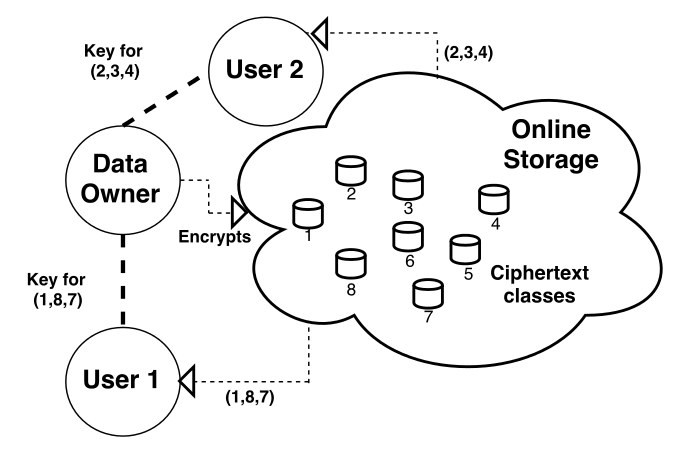
\includegraphics[scale=0.25]{Figs/KeyAgg.png}
\caption{Example of Online Data Sharing}
\label{fig:intro}
\end{figure}


\noindent{\textbf{Contributions:}} In this paper, we propose a basic key-aggregate scheme on additive elliptic subgroups that delegate decryption rights to multiple ciphertext classes using a single constant sized key. The scheme is dynamic in nature, that is, it allows the data owner to revoke access rights of users without having to change the entire set-up, unlike in the existing KAC scheme.  We then generalize this scheme into a two-level construction that allows flexible public key extension and maintains constant ciphertext size, while avoiding many of the pitfalls of earlier hierarchical schemes. We provide a formal proof of semantic security for the generalized scheme. We further extend the generalized scheme to allow using popular and efficiently implementable elliptic curve pairing schemes. We compare the time and space requirements of the proposed generalized scheme under various operating configurations. We also compare the performance of our proposed scheme, in terms of key size and resource 
utilization, with that of other existing schemes in literature.

\noindent{\textbf{Organization:}} The rest of the paper is organized as follows. Section \ref{sec:relwork} provides a brief overview of state of the art data sharing schemes. Section \ref{sec:prelims} introduces the notion of key aggregate cryptosystem, and provides a description of the complexity assumptions used to prove the semantic security of our proposed schemes. Our basic dynamic key-aggregate scheme is presented in Section \ref{sec:proposal}. We follow up with a more generalized two-tiered construction of the scheme for efficient public key extension in Section \ref{sec:general}, and prove its semantic security. A further extension for the generalized scheme that allows using efficiently implementable pairings is introduced and proved semantically secure in Section \ref{sec:extended}. Experimental results using Tate pairings based implementations of the extended scheme are presented in Section \ref{sec:results}. Finally Section \ref{sec:conclusions} concludes the paper.  



\section{Related Work}
\label{sec:relwork}

In this section we present a brief overview of public and private key cryptographic schemes in literature for secure online data sharing. While many of them focus on key aggregation in some form or the other, very few have the ability to provide constant size keys to decrypt an arbitrary number of encrypted entities.

\subsection{Hierarchical Encryption}
\label{subsec:hierarchy}

One of the most popular techniques for access control in online data storage is to use a pre-defined hierarchy of secret keys \cite{akl1983cryptographic,chick1990flexible,tzeng2002time,ateniese2012provably} in the form of a tree-like structure, where access to the key corresponding to any node implicitly grants access to all the keys in the subtree rooted at that node. For instance, \cite{sandhu1988cryptographic} uses repeated evaluations of a pseudo-random function/block cipher on a fixed secret to generate a tree hierarchy of symmetric keys. Some more advanced schemes \cite{sun2004scalable,king2015centralized,atallah2009dynamic} extend access control to cyclic and acyclic graphs. A major disadvantage of hierarchical encryption schemes is that granting access to only a selected set of branches within a given subtree warrants an increase in the number of granted secret keys. This in turn blows up the size of the key shared. Thus while hierarchical cryptosystems provide a neat key delegation mechanism when 
all files in a given branch is to be shared, its efficiency drops drastically as the complexity of the delegation increases.

\subsection{Compact Key Symmetric Encryption}
\label{subsec:symmetric}

Compact key encryption for the symmetric key setting has been used in \cite{benaloh2009patient,benaloh2009key} to solve the problem of concisely transmitting  large number of keys in the broadcast scenario. The basic methodology is to divide the entire ciphertext space into a finite set of classes, followed by a constant size aggregate key generation for the set of classes to be delegated. This scheme thus solves the problem of multi-class delegation faced by hierarchical schemes. However, symmetric key sharing via a secured channel is costly and not always practically viable for many applications on the cloud. Some other schemes in the symmetric key setting also attempt to reduce the key size \cite{alomair2009information}, but they are not aimed at decryption key delegation and are hence not very relevant to the present discussion.

\subsection{Compact Key Identity-Based Encryption}
\label{subsec:IBE}

Identity-Based Encryption (IBE) is a public key-based encryption scheme in which the public key for any user is an identity-string corresponding to that user. Proposed initially in \cite{shamir1985identity}, IBE was concretized by the proposition of two very widely cited and popular IBEs - The Boneh-Franklin scheme  \cite{boneh2003identity} and Cocks' encryption scheme \cite{cocks2001identity}. An IBE system comprises of a trusted private key generator that holds a master-secret key and issues a secret key to each user based on the user identity. Each user receives a message that has been encrypted using her id and some public parameters, and can decrypt the same using the secret key allotted to her by the trusted party. Compact key IBEs have been proposed in \cite{guo2007identity} and \cite{guo2008multi}. The former approach involves the use of random oracles while the latter shuns the use of oracles. Both these schemes allow aggregation of keys; however each key must come from a different identity division.
 Fuzzy IBE \cite{sahai2005fuzzy} allows for a single compact key to decrypt multiple ciphertexts, but they must have been encrypted under a closed set of identities, and the scheme does not work in practical scenarios for arbitrary identities. 

\subsection{Attribute Based Encryption}
\label{subsec:ABE}

Attribute-based encryption (ABE) \cite{goyal2006attribute,bethencourt2007ciphertext,chase2007multi} allows each user to be identified by a set of attributes. An encrypted file stored in cloud can only be decrypted by an user who has access to the corresponding secret key. The secret key is securely transmitted to the user who satisfies the access control policies set by the data owner. A major drawback of this scheme is that each time the access right to a particular user is revoked the entire ciphertext has to be recrypted in the cloud. The idea of ABE has been extended to shared keys for user groups in \cite{li2013scalable} with the focus on collusion resistance and not on key size compression.  

\subsection{Proxy Re-Encryption}
\label{subsec:PBE}

Proxy re-encryption is another technique to achieve fine-grained access control and scalable user revocation in unreliable clouds \cite{ateniese2006improved}. In this method the data owner and a semi trusted proxy cloud share a secret key in advance, with which the cloud can be delegated to re-encrypt data on behalf of the data owner. The semi-trusted proxy re-encrypts the data using the data owner's public key, thus converting it into a file that can in turn be decrypted by the secret key of the client. In the whole process, the proxy has no knowledge of the data being sent. An extension to this technique has been proposed in \cite{liu2011reliable} that allows the cloud servers to automatically re-encrypt data based on their internal clocks, without any external trigger. However, proxy re-encryption essentially transfers the responsibility for secure key storage from the delegatee to the proxy and is susceptible to collusion attacks. It is also important to ensure that the transformation key of the proxy is 
well protected, and every decryption would require a separate interaction with the proxy, which is inconvenient for applications on the cloud.

\subsection{Key-Aggregate Cryptosystems (KAC)}
\label{subsec:aggregate}

The authors of \cite{chu2014key} proposes an efficient scheme, namely KAC, that allows secure and efficient sharing of data on the cloud. The scheme is a public-key cryptosystem that uses constant size ciphertexts such that efficient delegation of decryption rights for any set of ciphertexts are possible. When a user demands for a particular subset of the available classes of data, the data owner computes an aggregate key which integrates the power of the individual decryption keys corresponding to each class of data. However, KAC as proposed in \cite{chu2014key} suffers from three major drawbacks, each of which we address in this paper. First of all, the security assumption of KAC seems to be the Bilinear Diffie Hellman Exponent (BDHE) assumption \cite{miller1986use}; however no concrete proofs of semantic security are provided by the authors in \cite{chu2014key}. Secondly, with respect to user access rights, KAC is a static scheme in the sense that once a user is in possession of the aggregate key corresponding to a subset of files from data owner, the owner cannot dynamically revoke the permission of the client for accessing one or more updated files. Since dynamic changes in access rights is extremely common in online data storage, this scenario needs to be tackled. Finally, the public key extension of KAC proposed in \cite{chu2014key} is extremely cumbersome and resource consuming since registration of each new public key-private key pair requires the number of classes to be extended by the original number of classes. 







\section{Preliminaries}
\label{sec:prelims}

In this section, we formally define the key-aggregate cryptosystem~(KAC) framework as well its security. For clarity of understanding, we present the definition in two parts. The first part defines a basic KAC framework that focuses on generating small aggregate keys for arbitrarily large subsets of data classes. The second part extends this basic framework by combining it with broadcast encryption systems to distribute the aggregate key among multiple data users.

\subsection{Key-Aggregate Cryptosystem : The Basic Version}
\label{subsec:basic_framework}

The basic KAC is an ensemble of five poly-time randomized algorithms that are described next:\\

\noindent\textbf{SetUp}($\mathcal{ID}$): A data owner can classifying her data into one or more classes belonging an identity space $\mathcal{ID}$. The function sets up the key-aggregate cryptosystem for the identity space $\mathcal{ID}$. Outputs the public parameter $param$. \\

\noindent\textbf{KeyGen}(): Outputs a master-secret key $msk$ and the corresponding public key $PK$. A unique tuple $(msk,PK)$ is generated for each data owner.\\ 

\noindent\textbf{Encrypt}$(param,PK,i,\mathcal{M})$: Takes as input the public key parameter $PK$, the data class $i\in\mathcal{ID}$ and the plaintext message $\mathcal{M}$. Outputs the corresponding ciphertext $\mathcal{C}$, which is stored online in the shared environment.\\

\noindent\textbf{Extract}$(param,msk,\mathcal{S})$: Takes as input the master secret key and a polynomial size subset of data classes $\mathcal{S} \subseteq\mathcal{ID}$. Computes the aggregate key $K_{\mathcal{S}}$ for all encrypted data/messages classified into any class in $\mathcal{S}$.\\

\noindent\textbf{Decrypt}$(param,\mathcal{C},i,\mathcal{S},K_{\mathcal{S}})$: Takes as input the ciphertext $\mathcal{C}$, the data class $i$ and the aggregate key $K_{\mathcal{S}}$ corresponding to a subset $\mathcal{S}$. If $i\notin\mathcal{S}$, output $\bot$. Otherwise, outputs the decrypted message $\mathcal{M}$. The \textbf{Decrypt} function is invoked by a data user with the appropriate credentials to access one or more classes of data owned by the data owner. Note that the \textbf{Decrypt} operation for a given data user requires the explicit knowledge of the subset $\mathcal{S}$ of data classes that the corresponding user can access. This is of course a valid requirement since each user is expected to be aware of the subset $\mathcal{S}$ of data classes that she can access.

\subsubsection{Correctness.} For correctness, we require that the decryption algorithm always succeeds in decrypting a correctly encrypted plaintext message $m$. Formally, correctness of KAC may be described as follows. For any valid identity space $\mathcal{ID}$, any set $\mathcal{S}\subseteq\mathcal{ID}$, any index $i\in\mathcal{S}$, and any plaintext message $m$, we must have 
\begin{equation}
 Pr[\textbf{Decrypt}(\mathcal{C},i,\mathcal{S},K_{\mathcal{S}})=\mathcal{M} |\mathcal{E}]=1\nonumber
\end{equation}
where $\mathcal{E}$ is the event described as the conjunction of the following atomic events:
\begin{equation}
\begin{split}
param\leftarrow\textbf{SetUp}(\mathcal{ID}),(msk,PK)\leftarrow\textbf{KeyGen}(),\\
\mathcal{C}\leftarrow\textbf{Encrypt}(param,PK,i,\mathcal{M}),K_{\mathcal{S}}\leftarrow\textbf{Extract}(msk,\mathcal{S})\nonumber
\end{split} 
\end{equation}


\subsection{Security Definitions}
\label{subsec:security}

We define a formal framework for proving active chosen ciphertext security of KAC. We begin by introducing a game between a non-adaptive attack algorithm $\mathcal{A}$ and a challenger $\mathcal{B}$, both of whom are given $\mathcal{ID}$, the data class identity space, as input. The game proceeds through the following stages.\\
 
\noindent\textbf{SetUp}: Challenger $\mathcal{B}$ sets up the KAC system. In particular, $\mathcal{B}$ generates the public parameter $param$, the master secret key $msk$ and the public key $PK$. Of these, $param$ and $PK$ are furnished to $\mathcal{A}$.\\
 
\noindent\textbf{Query Phase 1}: Algorithm $\mathcal{A}$ adaptively issues decryption queries $q_1,\cdots,q_w$. Here a decryption query comprises of the tuple $(\mathcal{C},v)$, where $v\in\mathcal{ID}$ is the data class of the message encrypted as $\mathcal{C}$. The challenger has to respond a valid decryption of the ciphertext.\\
 
\noindent\textbf{Commit:} $\mathcal{A}$ adaptively commits to a set $\mathcal{S} \subset \mathcal{ID}$ of data classes that it wishes to attack. Since collusion attacks are allowed in our framework, $\mathcal{B}$ furnishes $\mathcal{A}$ with the aggregate key $K_{\overline{\mathcal{S}}}$ that allows $\mathcal{A}$ to decrypt any data class $v\notin\mathcal{S}$. Next, $\mathcal{B}$ randomly chooses a data class $i\in\mathcal{S}$ and provides it to $\mathcal{A}$.\\ 
 
\noindent\textbf{Challenge}: $\mathcal{A}$ picks at random two messages $\mathcal{M}_0$ and $\mathcal{M}_1$ from the set of possible plaintext messages and provides them to $\mathcal{B}$. To generate the challenge, $\mathcal{B}$ randomly picks $b\in\{0,1\}$, and sets the challenge to $\mathcal{A}$ as $(\mathcal{C}^{*},\mathcal{M}_0,\mathcal{M}_1)$, where ${\mathcal{C}}^{*}$ = \textbf{Encrypt}($PK,i,\mathcal{M}_b$).\\
 
\noindent\textbf{Query Phase 2}: $\mathcal{A}$ continues to adaptively issue decryption queries $q_{w+1},\cdots,q_{Q_D}$ where a decryption query comprises of the tuple $(\mathcal{C},v)$, but is now subject to the restriction $\mathcal{C}\neq {\mathcal{C}}^{*}$. $\mathcal{B}$ responds as in query phase 1.\\ 
 
 
\noindent\textbf{Guess}: $\mathcal{A}$ outputs a guess $b'$ of $b$. If $b' = b$, $\mathcal{A}$ wins the game.\\

% Note that the adversary $\mathcal{A}$ is non-adaptive; it chooses $\mathcal{S}$, and obtains the aggregate decryption key for all data classes outside of $\mathcal{S}$, before it even sees the public parameters $param$ or the public key $PK$

% \vspace{-2mm}
\noindent The game above models an attack in the real world setting where users who do not have authorized access to the subset $\mathcal{S}$ collude to try and expose a message in this subset. We now formally define the security notions for KAC. Let $Adv_{\mathcal{A},|\mathcal{ID}|}$ denote the probability that $\mathcal{A}$ wins the game.
\subsubsection{Definition 2.1.}
 A KAC construction is $(\epsilon,\mathcal{ID},Q_D)$ adaptively secure under a chosen ciphertext attack (that is, adaptively CCA-secure) if, for all adaptive probabilistic ploy-time algorithms $\mathcal{A}$ that can make a total of $Q_D$ decryption queries, we have that $|Adv_{\mathcal{A},|\mathcal{ID}|}-\frac{1}{2}| < \epsilon$.
 
\subsubsection{Definition 2.2.}
 A KAC construction is $(\epsilon,\mathcal{ID})$ adaptively secure under a chosen plaintext attack (that is, adaptively CPA-secure) if it is $(\epsilon,\mathcal{ID},0)$ adaptively CCA secure.\\


\noindent We also define two weaker notions of security in the non-adaptive setting. In particular, non-adaptive security is achieved in the scenario when $\mathcal{A}$ is required to commit to the set $\mathcal{S}$ before seeing the public parameters. We refer to such an adversary as a non-adaptive adversary. This leads to the following definitions.

\subsubsection{Definition 2.3.}
 A KAC construction is $(\epsilon,\mathcal{ID},Q_D)$ non-adaptively secure under a chosen ciphertext attack (that is, non-adaptively CCA-secure) if, for all non-adaptive probabilistic ploy-time algorithms $\mathcal{A}$ that can make a total of $Q_D$ decryption queries, we have that $|Adv_{\mathcal{A},|\mathcal{ID}|}-\frac{1}{2}| < \epsilon$.
% \end{Definition}

\subsubsection{Definition 2.4.}
 A KAC construction is $(\epsilon,\mathcal{ID})$ non-adaptively secure under a chosen plaintext attack (that is, non-adaptively CPA-secure) if it is $(\epsilon,\mathcal{ID},0)$ non-adaptively CCA secure.
% \end{Definition}

\subsection{Extensions to The Basic Version : Broadcasting Aggregate Keys}
\label{subsec:extensions}

We discuss in this paper two extensions to the basic framework of KAC for a full-fledged public key based implementation in practical data sharing environments. We first note that the standalone KAC framework presented in Section \ref{subsec:basic_framework} is a perfectly suitable choice when a single data owner wishes to delegate access rights to a particular subset of her data to a given data user. However, any practically deployable online data sharing scheme must be able to support multiple data owners, who should in turn be able to delegate access rights to their data to multiple users. In this context, there are two major requirements that the standalone KAC framework does not explicitly cater to:

\begin{itemize}
 \item Data privacy must be ensured for each individual data owner. In particular, an aggregate decryption key issued by one data owner should not leak information about the data of another data owner to an unauthorized user.
 \item Distribution of aggregate keys to a large number of data users must be handled efficiently and, preferably, via a public key based protocol and not a secure channel as suggested in \cite{chu2014key}.
\end{itemize}

\noindent In this paper, we augment the basic KAC framework to tackle both these problems efficiently. In particular, the second problem is handled by combining the basic KAC framework with that of the identity-based broadcast encryption scheme proposed in \cite{boneh2014low}. We formally define the combined scheme, referred to as the \emph{extended} KAC framework, using the following set of algorithms. Note that $\mathcal{ID}_1$ and $\mathcal{ID}_2$ denote the identity spaces for the data classes and the data users respectively.\\

\noindent\textbf{SetUp}($\mathcal{ID}_1,\mathcal{ID}_2$): Same as the basic KAC framework. \\

\noindent\textbf{OwnerKeyGen}(): In addition to the public key $PK$ and the master-secret key $msk$, also outputs a distribution-secret key $dsk$. The tuple $(msk,PK,dsk)$ is made available to the data owner.\\ 

\noindent\textbf{Encrypt}$(param,PK,dsk,i,\mathcal{M})$: Takes as input the data class $i\in\mathcal{ID}_1$ and the plaintext message $\mathcal{M}$. Outputs the corresponding ciphertext $\mathcal{C}$.\\

\noindent\textbf{UserKeyGen}$(param,msk,\hat{i})$: Takes as input the index $\hat{i}\in\mathcal{ID}_2$ for a user and outputs the corresponding secret key $d_{\hat{i}}$.\\ 

\noindent\textbf{Extract}$(param,msk,\mathcal{S})$: Takes as input the master secret key and a polynomial size subset of data classes $\mathcal{S} \subseteq\mathcal{ID}_1$. Computes the aggregate key $K_{\mathcal{S}}$ for all encrypted data/messages classified into any class in $\mathcal{S}$.\\

\noindent\textbf{Broadcast}$(param,K_{\mathcal{S}},\hat{\mathcal{S}},PK,dsk)$: Takes as input the aggregate key $K_{\mathcal{S}}$, the polynomial size target subset of users $\hat{\mathcal{S}}\subseteq\mathcal{ID}_2$. Outputs a single \emph{broadcast aggregate key} $K_{\left(\mathcal{S},\hat{\mathcal{S}}\right)}$ that allows any user $\hat{i}\in\hat{\mathcal{S}}$ to decrypt all encrypted data/messages classified into any class $i\in\mathcal{S}$.\\

\noindent\textbf{Decrypt}$(param,\mathcal{C},K_{\left(\mathcal{S},\hat{\mathcal{S}}\right)},i,\hat{i},d_{\hat{i}},\mathcal{S},\hat{\mathcal{S}})$: The decryption algorithm now takes, besides the ciphertext $\mathcal{C}$ and the corresponding data class $i\in\mathcal{S}$, a valid user id $\hat{i}\in\hat{\mathcal{S}}$. It also takes as input the broadcast aggregate key $K_{\left(\mathcal{S},\hat{\mathcal{S}}\right)}$ and the secret key $d_{\hat{i}}$. The algorithm outputs the decrypted message.\\

% \noindent We avoid presenting separately the game-based security framework for the extended KAC scheme here. The framework is directly introduced when proving the security of our proposed construction in Section \ref{subsec:multiuserKAC}.

\subsection{Security of Extended KAC: A Game Based Framework}
\label{subsec:gameextended}

We also define the formal framework for proving the security of the extended KAC via the following game between an attack algorithm $\mathcal{A}$ and a challenger $\mathcal{B}$:\\

\noindent\textbf{SetUp}: Challenger $\mathcal{B}$ sets up the KAC system. In particular, $\mathcal{B}$ generates the public parameter $param$, the master secret key $msk$, the distribution secret key $dsk$ and the public key $PK$. Of these, $param$ and $PK$ are furnished to $\mathcal{A}$.\\
 
\noindent\textbf{Query Phase 1}: Algorithm $\mathcal{A}$ adaptively issues decryption queries $q_1,\cdots,q_w$. Here a decryption query comprises of the tuple $(\mathcal{C},v)$, where $v\in\mathcal{ID}$ is the data class of the message encrypted as $\mathcal{C}$. The challenger has to respond a valid decryption of the ciphertext.\\
 
\noindent\textbf{Commit:} $\mathcal{A}$ adaptively commits to a set $\mathcal{S} \subset \mathcal{ID}_1$ of data classes and a corresponding set $\hat{\mathcal{S}} \subset \mathcal{ID}_2$ of authorized data users (with access to $\mathcal{S}$) that it wishes to attack. Since collusion attacks are allowed in our framework, $\mathcal{B}$ furnishes $\mathcal{A}$ with all the private user keys $d_{\hat{j}}$ for $\hat{j}\notin\hat{\mathcal{S}}$. In addition, $\mathcal{A}$ is also provided with the broadcast aggregate key $K_{\left(\overline{\mathcal{S}},\hat{\mathcal{S}}\right)}$ that allows any user in $\hat{\mathcal{S}}$ to decrypt any ciphertext class $v\notin{\mathcal{S}}$.\\  
 
\noindent\textbf{Challenge}: $\mathcal{A}$ picks at random two messages $\mathcal{M}_0$ and $\mathcal{M}_1$ from the set of possible plaintext messages and provides them to $\mathcal{B}$. To generate the challenge, $\mathcal{B}$ randomly picks $b\in\{0,1\}$, and sets the challenge to $\mathcal{A}$ as $(\mathcal{C}^{*},\mathcal{M}_0,\mathcal{M}_1)$, where ${\mathcal{C}}^{*}$ = \textbf{Encrypt}($PK,i,\mathcal{M}_b$).\\
 
\noindent\textbf{Query Phase 2}: $\mathcal{A}$ continues to adaptively issue decryption queries $q_{w+1},\cdots,q_{Q_D}$ where a decryption query comprises of the tuple $(\mathcal{C},v)$, but is now subject to the restriction $\mathcal{C}\neq {\mathcal{C}}^{*}$. $\mathcal{B}$ responds as in query phase 1.\\

\noindent\textbf{Guess}: $\mathcal{A}$ outputs a guess $b'$ of $b$. If $b' = b$, $\mathcal{A}$ wins the game.\\

The game above models an attack involving two different kinds of collusion. The first collusion is by all users not in $\hat{\mathcal{S}}$ who collude to try and expose an aggregate key that is broadcast for users in $\hat{\mathcal{S}}$ only. The second collusion is by users in $\hat{\mathcal{S}}$ who collude (by compromising the knowledge of the aggregate key for different subsets) to try and expose a message class in $\mathcal{S}$.

We next define the security of extended KAC. Let $Adv'_{\mathcal{A},|\mathcal{ID}_1|,|\mathcal{ID}_2|}$ denote the probability that $\mathcal{A}$ wins the above game.

\subsubsection{Definition 2.5.}
An extended KAC construction with the ability to broadcast aggregate keys is $(\epsilon,mathcal{ID}_1,\mathcal{ID}_2,Q_D)$ non-adaptively secure under a chosen ciphertext attack (that is, non-adaptively CCA-secure) if, for all non-adaptive probabilistic ploy-time algorithms $\mathcal{A}$ that can make a total of $Q_D$ decryption queries, we have that $|Adv'_{\mathcal{A},|\mathcal{ID}_1|,|\mathcal{ID}_2|}-\frac{1}{2}| < \epsilon$.
% \end{Definition}

\subsubsection{Definition 2.6.}
An extended KAC construction is $(\epsilon,\mathcal{ID}_1,\mathcal{ID}_2)$ non-adaptively secure under a chosen plaintext attack (that is, non-adaptively CPA-secure) if it is $(\epsilon,\mathcal{ID}_1,\mathcal{ID}_2,0)$ non-adaptively CCA secure.
 

\subsection{Multilinear Maps}
\label{subsec:multilinear}

In this section, we provide a brief overview of multilinear maps. Our description of multilinear maps is based on the \emph{graded encoding scheme} used in several candidate multilinear map constructions \cite{garg2013candidate}.

\subsubsection{Symmetric Multilinear Maps.} A standard symmetric multilinear map consists of the following pair of algorithms.\\

\noindent\textbf{SetUp}$'(1^\lambda,m)$: Sets up an $m$-linear map by outputting an $m$-tuple of groups $<\mathbb{G}_1,\mathbb{G}_2,\cdots,\mathbb{G}_m>$ of prime order $q$ (where $q$ is a $\lambda$ bit prime), along with the respective generator $g_i\in\mathbb{G}_i$ for $1\leq i\leq m$. In standard notation, $\mathbb{G}_1$ is the source group, $\mathbb{G}_m$ is the target group, and $\mathbb{G}_2,\cdots,\mathbb{G}_{m-1}$ are the intermediate groups.\\

\noindent$e_{i,j}(h_1,h_2)$: Takes as input $h_1\in\mathbb{G}_i$ and $h_2\in\mathbb{G}_j$, and outputs $h_3\in\mathbb{G}_{i+j}$ such that
\begin{equation}
 (h_1=g_i^a,h_2=g_j^b) \Rightarrow h_3=g_{i+j}^{ab}\nonumber
\end{equation}
\noindent In this paper, we follow the standard notation used in the literature to omit the subscripts and simply refer to this multilinear map as $e$. Further, $e$ may be generalized to multiple inputs as $e(h_1,\cdots,h_k)=e(h_1,e(h_2,\cdots,h_k))$. Note that $g^a_i$ is sometimes referred to as the level-$i$ \emph{encoding} of $a$. The scalar $a$ itself may therefore be referred to as the level $0$ encoding of itself.

\subsubsection{Asymmetric Multilinear Maps.} We adopt the same definition of asymmetric multilinear maps presented in \cite{garg2013candidate}. According to this definition, in asymmetric multilinear maps, the groups are indexed by integer vectors. Formally, a standard asymmetric multilinear map consists of the following algorithms.\\

\noindent\textbf{SetUp}$''(1^\lambda,\mathbf{m})$: Takes as input $\mathbf{m}\in\mathbb{Z}^l$. Sets up an $\mathbf{m}$-linear map by outputting an $m$-tuple of groups $<\mathbb{G}_{\mathbf{1}},\mathbb{G}_{\mathbf{2}},\cdots,\mathbb{G}_{\mathbf{m}}>$ of prime order $q$ (where $q$ is a $\lambda$ bit prime), along with the respective generator $g_{\mathbf{v}}\in\mathbb{G}_{\mathbf{v}}$ for $\mathbf{1}\leq \mathbf{v}\leq \mathbf{m}$(comparison is defined component-wise). Further, let $\mathbf{x}_i$ be the $i$th \emph{standard} basis vector (with $1$ at position $i$ and $0$ at each other position). In standard notation, $\mathbb{G}_{\mathbf{x}_i}$ is the $i$th source group, $\mathbb{G}_{\mathbf{v}}$ is the target group, and the rest are the intermediate groups.\\

\noindent$e_{\mathbf{i},\mathbf{j}}(h_1,h_2)$: Takes as input $h_1\in\mathbb{G}_\mathbf{i}$ and $h_2\in\mathbb{G}_\mathbf{j}$, and outputs $h_3\in\mathbb{G}_\mathbf{i+j}$ such that
\begin{equation}
 (h_1=g_\mathbf{i}^a,h_2=g_\mathbf{j}^b)\Rightarrow h_3=g_\mathbf{i+j}^{ab}\nonumber
\end{equation}
\noindent Again, we omit the subscripts and simply refer to this multilinear map as $e$, which may be generalized to multiple inputs as $e(h_1,\cdots,h_k)=e(h_1,e(h_2,\cdots,h_k))$.\\ 

In the forthcoming discussions, we present our KAC constructions assuming that the ideal multilinear maps based on the graded encoding scheme described above exist and are efficiently computable. We do this to make the analysis simple and easy to follow. We point out, however, that current candidates for multilinear maps in the cryptographic literature deviate from these ideal notions. In these candidates, group elements lack unique representations due to the presence of a noise term that tends to grow with repeated group/multilinear operations. However, as pointed out in \cite{boneh2014low}, most candidate constructions \cite{garg2013candidate,coron2013practical,gentry2014zeroizing,boneh2014immunizing} possess the necessary properties to instantiate public key constructions based on ideal multilinear maps. Unfortunately, most of these constructions have been cryptanalyzed \cite{cheon2015cryptanalysis,coron2014cryptanalysis}. To the best of our knowledge, the foremost candidate construction for multilinear maps currently unbroken is the graph-induced multilinear map based on lattices proposed by Gentry et al. \cite{gentry2015graph}, which naturally gives rise to asymmetric multilinear maps. We point out that it is possible to instantiate our KAC constructions using this candidate map since it meets our requirements listed below:

\let\labelitemi\labelitemii

\begin{itemize}
 \item The representation of an element should be statistically independent of the group and multilinear operations that led to that element. This is achieved using Kilian-style randomization \cite{kilian1988founding} on the encoding side \cite{gentry2015graph}.\\
 \item It is possible to extract a \emph{canonical} representation of an element in the target group given any representation of that element using the \emph{zero-test parameter}.\\
 \item The party setting up the multilinear map has sufficient \emph{trapdoor} information to compute $g^{\alpha^x}$ for a non-random $\alpha$ and exponentially large $x$.\\
 \item It is possible to generate asymmetric multilinear maps for any positive integer vector $\mathbf{m}\in\mathbb{Z}^l$.\\
%  \item It should be possible to design the parameters of our system such that the noise growth during the execution of our scheme does not lead to erroneous computations. 
\end{itemize}

\noindent However, in order to successfully instantiate our proposed schemes using graph induced multilinear map candidates, it is important to ensure that the algebraic elements used in our constructions are suitably encoded as paths in a directed graph and adequate precautions are taken to prevent weak trapdoor attacks.  

% We point out that the two foremost candidates for multilinear maps based on graded encoding schemes - the GGH candidate over ideal lattices \cite{garg2013candidate} and the CLT candidate over integers \cite{coron2013practical} would allow us to meet all these requirements. However, we also note that both these candidate constructions have been subjected to \emph{zeroizing attacks}\cite{cheon2015cryptanalysis}, also known as the weak discrete logarithmic attack. These attacks break the Subgroup Membership (SubM) and the decision linear (DLIN) problems on the GGH candidate map, and also completely break the CLT candidate. Initially it was conjectured that this attack could be thwarted by keeping the low-level encodings of $0$ private in the candidate constructions, and several fixes to these candidate constructions were provided based on this idea \cite{gentry2014zeroizing,boneh2014immunizing}. However, these extensions were also proven to be insecure in \cite{coron2014cryptanalysis}. 
% 
% In this paper, we propose using use the graph-induced multilinear map based on lattices proposed by Gentry et al. \cite{gentry2015graph} to instantiate our constructions. The graph-induced multilinear map, like the GGH and CLT candidate constructions, is also based on the graded encoding scheme and meets almost all the requirements listed above. The only significant drawback of this construction is the absence of the \emph{re-randomization} procedure (that helps to hide the group and multilinear operations leading to a particular element) to thwart cryptanalytic threats. However, a work around suggested in \cite{gentry2015graph} is to use Kilian-style randomization \cite{kilian1988founding} on the encoding side. This enhances the security of any scheme based on the graph induced candidate map, at the cost of some extra encoding bits.




% \noindent\textbf{The Multilinear Diffie-Hellman Exponent (MDHE) Assumption}:  Let $param\leftarrow SetUp'(n+l-1)$. Choose random 


 









\section{The Proposed Dynamic Key-Aggregate Cryptosystem: The Basic Case}
\label{sec:proposal}

In this section, we present the design of our proposed dynamic key-aggregate storage scheme on additive elliptic curve subgroups assuming that there are $n$ ciphertext classes. Our scheme ensures that the ciphertext and aggregate key are of constant size, while the public parameter size is linear in the number of ciphertext classes. Unlike the scheme proposed in \cite{chu2014key}, the proposed scheme allows dynamic revocation of user access rights without having to massively change the system parameters. We also present a proof of security for the proposed scheme.

\subsection{The Basic Construction of Dynamic KAC}
\label{subsec:construction1}

Let $\mathbb{G}$ be an additive cyclic elliptic curve subgroup of prime order $q$, where $2^{\lambda}\leq q \leq 2^{\lambda + 1}$, such that the point $P$ is a generator for $\mathbb{G}$. Also, let $\mathbb{G}_{T}$ be a multiplicative group of order $q$ with identity element $1$. We assume that there exists an efficiently computable bilinear pairing $\hat{e'}:\mathbb{G} \times \mathbb{G}\longrightarrow\mathbb{G}_T$. We now present the basic construction of our proposed key-aggregate encryption scheme. 

The scheme consists of the following five phases.

\begin{enumerate}
 \item \textbf{Setup}$(1^{\lambda},n)$: Randomly pick $\alpha \in \mathbb{Z}_q$. Compute $P_i = {\alpha^{i}}P \in \mathbb{G}$ for $i = 1,\cdots,n,n+2,\cdots,2n$. Output the system parameter as\\
 $param = (P,P_1,\cdots,P_n,P_{n+2},\cdots,P_{2n})$. The system also randomly chooses a secret parameter $t \in \mathbb{Z}_q$ which is not made public. It is only known to data owners with credentials to control client access rights.
 \item \textbf{Keygen}(): Pick $\gamma \in \mathbb{Z}_q$, output the public and master-secret key pair : \\$(PK={\gamma}P,msk=\gamma)$.
 \item \textbf{Encrypt}$(PK,i,m)$: For a message $m \in \mathbb{G}_T$ and an index $i \in \{1,2,\cdots,n\}$, randomly choose $r\in\mathbb{Z}_q$ and let $t'=t+r \in\mathbb{Z}_q$. Then the ciphertext is computed as\\ $\mathcal{C}=(rP,t'{(PK+P_i)},m.\hat{e'}(P_n,t'P_1))$ $=$ $(c_1,c_2,c_3)$
 \item \textbf{Extract}$(msk=\gamma,\mathcal{S})$: For the set $\mathcal{S}$ of indices $j$ the aggregate key is computed as\\ $K_{\mathcal{S}} = \sum_{j\in\mathcal{S}}{\gamma}P_{n+1-j}$ = $\sum_{j\in\mathcal{S}}\alpha^{n+1-j}PK$\\ and the dynamic access control parameter $U$ is computed as $tP$. Thus the net aggregate key is $(K_{\mathcal{S}},U)$ which is transmitted via a secure channel to users that have access rights to $\mathbb{S}$.
 \item \textbf{Decrypt}$(K_{\mathcal{S}}, U, \mathcal{S},i,\mathcal{C}=\{c_1,c_2,c_3\})$: If $i\notin\mathcal{S}$, output $\bot$. Otherwise return the message\\ $\hat{m}=c_3\hat{e'}(K_{\mathcal{S}}+\sum_{j\in\mathcal{S},j\neq i}P_{n+1-j+i},U+c_1)/(\hat{e'}(\sum_{j\in\mathcal{S}}P_{n+1-j},c_2))$. 
\end{enumerate}

The proof of correctness of this scheme is presented below.

\begin{scriptsize}
\begin{equation*}
\label{eq:correctness}
\begin{split}
 \hat{m} &= c_3\frac{\hat{e'}(K_{\mathcal{S}}+\sum_{j\in\mathcal{S},j\neq i}P_{n+1-j+i},U+c_1)}{\hat{e'}(\sum_{j\in\mathcal{S}}P_{n+1-j},c_2)}\\
%   &= c_3\frac{\hat{e'}(\sum_{j\in \mathcal{S}}{\gamma}P_{n+1-j} + \sum_{j\in\mathcal{S},j\neq i}P_{n+1-j+i},t'P)}{\hat{e'}(\sum_{j\in\mathcal{S}}P_{n+1-j},t'(PK+P_i))}\\
  &= c_3\frac{\hat{e'}(\sum_{j\in \mathcal{S}}{\gamma}P_{n+1-j},t'P)\hat{e'}(\sum_{j\in\mathcal{S}}(P_{n+1-j+i})-P_{n+1},t'P)}{\hat{e'}(\sum_{j\in\mathcal{S}}P_{n+1-j},t'PK)\hat{e'}(\sum_{j\in\mathcal{S}}P_{n+1-j},t'P_i))}\\
%   &= c_3\frac{\hat{e'}(\sum_{j\in\mathcal{S}}P_{n+1-j+i},t'P)}{\hat{e'}(P_{n+1},t'P)\hat{e'}(\sum_{j\in\mathcal{S}}P_{n+1-j},t'P_i))}\\
  &= c_3\frac{\hat{e'}(\sum_{j\in\mathcal{S}}P_{n+1-j+i},t'P)}{\hat{e'}(P_{n+1},t'P)\hat{e'}(\sum_{j\in\mathcal{S}}P_{n+1-j+i},t'P))}\\
%   &= m\frac{\hat{e'}(P_n,t'P_1)}{\hat{e'}(P_{n+1},t'P)}\\
  &= m
\end{split}  
\end{equation*}
\end{scriptsize}


\subsection{Dynamic Access Control}
\label{subsec:dynamic}

An important aspect of the proposed scheme is the fact that it allows the data owner to dynamically update user access permissions. In KAC \cite{chu2014key}, once the data owner issues an aggregate key corresponding to a set of ciphertext classes to a user, revoking the user's access permissions to the same is not possible without changing the master secret key. However, changing the master secret key each time an user's access privileges to a ciphertext class need to be updated, is a very expensive option and may not be practically feasible. Our scheme, on the other hand, offers a solution to this problem by allowing the data owner to dynamically update user access privileges.

We achieve this by making the parameter $U=tP$ a part of the aggregate key in our proposed scheme and not a part of the ciphertext. The user must have the correct value of $U$ in possession to be able to decrypt any encrypted ciphertext class in the subset $\mathcal{S}$. Now suppose the data owner wishes to alter the access rights to the subset $\mathcal{S}$. She can simply re-encrypt all ciphertexts in that class using a different random element $\hat{t}\in\mathbb{Z}_q$, and then provide the updated dynamic access parameter $\hat{U}=\hat{t}P$ to only those users who she wishes to delegate access to. The decrypted value will give the correct message $m$ only if the same $t$ is used for both encryption and decryption. This is a major difference between our scheme and the scheme proposed in \cite{chu2014key}, where the knowledge of the random parameter was only embedded as part of the ciphertext itself, and could not be used to control access rights of users. Moreover, since $U$ is of constant size and needs to be transmitted only when changed (and not for every encryption), there is no significant degradation in performance.

\subsection{Performance and Efficiency}
\label{subsec:perf}
The decryption time for any subset of ciphertext classes $\mathcal{S}$ is essentially dominated by the computation of $W_{\mathcal{S}}=\sum_{j\in\mathcal{S}}P_{n+1-j+i}$. However, if a user has already computed $\sum_{j\in\mathcal{S}'}P_{n+1-j+i}$ for a subset $S'$ similar to $S$, then she can easily compute the desired value by at most $|\mathcal{S}-\mathcal{S}'|$ operations. For similar subsets $S$ and $S'$, this value is expected to be fairly small. A suggested in \cite{boneh2005collusion}, for subsets of very large size($n-r, r\ll n$), an advantageous approach could be to pre-compute $\sum_{j=1}^{j=n}P_{n+1-j+i}$ corresponding to $i=1$ to $n$, which would allow the user to decrypt using only $r$ group operations, and would require only $r$ elements of $param$. Similar optimizations would also hold for the encryption operation where pre-computation of  $\sum_{j=1}^{j=n}P_{n+1-j}$ is useful for large subsets.

It is important to note that our proposed scheme fixes the number of ciphertext classes beforehand, thus limiting the scope for ciphertext class extension. The only way to increase the number of classes is to change the public key parameters, which would therefore require some kind of administrative privileges, and cannot be done by an user for her own purposes. However, in online data sharing environments, users may wish to register their own public key-private key pairs for new ciphertext classes according to their own requirements. Such an extension to the scheme would make extremely convenient and attractive to potential users. A proposal made in \cite{chu2014key} recommends that the user be allowed to register new public-private key pairs, at the cost of increasing the number of ciphertext classes by $n$ each time. This is both impractical and wasteful. In the next section, we present a two-tier generalization of our scheme that tackles this issue in a more economical fashion. We avoid a separate proof of semantic security for the base case presented here, since the proof is a special case of the proof for the generalized scheme presented in the next section.  
  



\section{A Generalized Version of Dynamic KAC}
\label{sec:general}

In this section, we focus on building an efficiently extensible version of our proposed scheme that allows an user to economically increase the number of ciphertext classes while registering a new public key-private key pair. We adopt the idea presented in \cite{boneh2005collusion} to develop a hierarchical structure that has multiple instances (say $n_1$) of the original scheme running in parallel. Each such instance in turn provides \emph{locally aggregate keys} for $n_2$ ciphertext sub-classes. Each ciphertext class thus now has a double index $(i_1,i_2)$ where $1\leq i_1 \leq n_1$ and $1\leq i_2 \leq n_2$. This allows the overall setup to handle $n=n_1n_2$ classes. However, it is important to note that all the instances can use the same public parameters. This interaction among the instances helps to largely improve performance. We further point out that while in \cite{boneh2005collusion}, the generalized construction offers a trade-off between the public parameter size and the ciphertext size, our 
generalized scheme actually reduces the public parameter size without compromising on the size of the ciphertext. Further, addition of a single new key increases the number of classes only by $n_2$ and not by $n$. Setting $n_2\ll n$ thus achieves significant improvement in performance over the existing proposal.


\subsection{The Construction of the Generalized KAC}
\label{subsec:construction2}

Let $n_2$ be a fixed positive integer. Our proposed $n_2$-generalized key-aggregate encryption scheme over elliptic curve subgroups is as described below. It may be noted that the bilinear additive elliptic curve sub-group $\mathbb{G}$ and the multiplicative group $\mathbb{G}_T$, as well as the pairing $\hat{e'}$ are the same as in the basic scheme. The algorithm sets up $n_1=\lfloor n/n_2\rfloor$ instances of the basic scheme, each of which handles $n_2$ ciphertext classes. The original scheme is thus a special case of the extended scheme with $n_1=1$ and $n_2=n$.


\begin{enumerate}
 \item \textbf{Setup}$(1^{\lambda},n_2)$: Randomly pick $\alpha \in \mathbb{Z}_q$. Compute $P_i$ = ${\alpha^{i}}P \in \mathbb{G}$ for $i = 1,\cdots,n_2,n_2+2,\cdots,2n_2$. Output the system parameter as\\
 $param$ = $(P,P_1,\cdots,P_{n_2},P_{n_2+2},\cdots,P_{2n_2})$. The system randomly chooses a secret parameter $t \in \mathbb{Z}_q$ which is not made public. It is only known to data owners with credentials to control client access rights.
 \item \textbf{Keygen}(): Pick $\gamma_1,\gamma_2,\cdots,\gamma_{n_1} \in \mathbb{Z}_q$, output the public and master-secret key pair :\\ $(PK$=$({pk}_1,pk_{2},\cdots,pk_{n_1})=(\gamma_1P,\gamma_2P,\cdots,\gamma_{n_1}P)$,$msk$=$(\gamma_1,\gamma_2,\cdots,\gamma_{n_1}))$.
 \item \textbf{Encrypt}$(pk_{i_1},(i_1,i_2),m)$: For a message $m \in \mathbb{G}_T$ and an index $(i_1,i_2) \in \{1,2,\cdots,n_1\}\times\{1,2,\cdots,n_2\}$, randomly choose $r\in\mathbb{Z}_q$ and let $t'=t+r \in\mathbb{Z}_q$. Then compute the ciphertext $\mathcal{C}$=$(rP,t'{(pk_{i_1}+P_{i_2})},m.\hat{e'}(P_{n_2},t'P_1))$ = $(c_1,c_2,c_3)$.
 \item \textbf{Extract}$(msk=\gamma,\mathcal{S})$: For the set $\mathcal{S}$ of indices $(j_1,j_2)$ the aggregate key is computed as $K_{\mathcal{S}}$ = $(k^{1}_{\mathcal{S}},k^{2}_{\mathcal{S}},\cdots,k^{n_1}_{\mathcal{S}})$ =\\$(\sum_{(1,j_2)\in\mathcal{S}}{\gamma_{1}}P_{n_2+1-j_2},\sum_{(2,j_2)\in\mathcal{S}}{\gamma_{2}}P_{n_2+1-j_2},\cdots,\sum_{(n_1,j_2)\in\mathcal{S}}{\gamma_{n_1}}P_{n_2+1-j_2})$\\ and the dynamic access control parameter $U$ is computed as $tP$. Thus the net aggregate key is $(K_{\mathcal{S}},U)$ which is transmitted via a secure channel to users that have access rights to $\mathbb{S}$. Note that  $k^{j_1}_{\mathcal{S}}=\sum_{(j_1,j_2)\in\mathcal{S}}\alpha^{n+1-j}pk_{j_1}$ for $j_1=1,2,\cdots,n_1$. 
 \item \textbf{Decrypt}$(K_{\mathcal{S}}, U, \mathcal{S},(i_1,i_2),\mathcal{C}=\{c_1,c_2,c_3\})$: If $(i_1,i_2)\notin\mathcal{S}$, output $\bot$. Otherwise return the message\\ $\hat{m}$ = $c_3\frac{\hat{e'}(k^{i_1}_{\mathcal{S}}+\sum_{(i_1,j_2)\in\mathcal{S},j_2\neq i_2}P_{n_2+1-j_2+i_2},U+c_1)}{\hat{e'}(\sum_{(i_1,j_2)\in\mathcal{S}}P_{n_2+1-j_2},c_2)}$. 
\end{enumerate}

The proof of correctness for the generalized scheme is presented below.

\begin{scriptsize}
\begin{equation}
\begin{split}
 \hat{m} &= c_3\frac{\hat{e'}(k^{i_1}_{\mathcal{S}}+\sum_{(i_1,j_2)\in\mathcal{S},j_2\neq i_2}P_{n_2+1-j_2+i_2},U+c_1)}{\hat{e'}(\sum_{(i_1,j_2)\in\mathcal{S}}P_{n_2+1-j_2},c_2)}\\
  &= c_3\frac{\hat{e'}(\sum_{(i_1,j_2)\in \mathcal{S}}{\gamma_{i_1}}P_{n_2+1-j_2} + \sum_{(i_1,j_2)\in\mathcal{S},j_2\neq i_2}P_{n_2+1-j_2+i_2},t'P)}{\hat{e'}(\sum_{(i_1,j_2)\in\mathcal{S}}P_{n_2+1-j_2},t'(pk_{i_1}+P_{i_2})}\\
  &= c_3\frac{\hat{e'}(\sum_{(i_1,j_2)\in \mathcal{S}}{\gamma_{i_1}}P_{n_2+1-j_2},t'P)\hat{e'}(\sum_{(i_1,j_2)\in\mathcal{S}}(P_{n_2+1-j_2+i_2})-P_{n_2+1},t'P)}{\hat{e'}(\sum_{(i_1,j_2)\in\mathcal{S}}P_{n_2+1-j_2},t'pk_{i_1})\hat{e'}(\sum_{(i_1,j_2)\in\mathcal{S}}P_{n_2+1-j_2},t'P_{i_2})}\\
  &= c_3\frac{\hat{e'}(\sum_{(i_1,j_2)\in\mathcal{S}}P_{n_2+1-j_2+i_2},t'P)}{\hat{e'}(P_{n_2+1},t'P)\hat{e'}(\sum_{(i_1,j_2)\in\mathcal{S}}P_{n_2+1-j_2},t'P_{i_2})}\\
  &= c_3\frac{\hat{e'}(\sum_{(i_1,j_2)\in\mathcal{S}}P_{n_2+1-j_2+i_2},t'P)}{\hat{e'}(P_{n_2+1},t'P)\hat{e'}(\sum_{(i_1,j_2)\in\mathcal{S}}P_{n_2+1-j_2+i_2},t'P)}\\
  &= m\frac{\hat{e'}(P_{n_2},t'P_1)}{\hat{e'}(P_{n_2+1},t'P)}\\
  &= m
\end{split}  
\end{equation}
\end{scriptsize}

\subsection{Semantic Security of the Generalized KAC}
\label{subsec:proof_general}

\subsubsection{The Reduced Generalized Scheme:}

As in the original scheme, we may analogously define a reduced version of the generalized encryption scheme. We note that once again, in the generalized scheme, the ciphertext $\mathcal{C}=(c_1,c_2,c_3)$ output by the $Encypt$ operation essentially embeds the value of $m$ in $c_3$ by multiplying it with $\hat{e'}(P_{n_2},tP_1)$. Consequently, the security of our proposed scheme is equivalent to that of a \emph{reduced} generalized key-aggregate encryption scheme that simply uses the reduced ciphertext $(c_1,c_2)$, the aggregate key $K_{\mathcal{S}}$ and the dynamic access parameter $U$ to successfully transmit and decrypt the value of $\hat{e'}(P_{n_2},t'P_1)=\hat{e'}(P_{n_2+1},t'P)$. We prove the semantic security of this \emph{reduced scheme} parameterized with a given number of ciphertext classes $n_2$ for each instance, which also amounts to proving the semantic security of our original encryption scheme for the same number of ciphertext classes. Note that the proof of security is independent of the 
number of instances $n_1$ that run in parallel. The adversarial model is the same as in the case of the proof for the basic scheme.

\subsubsection{The Security Proof:}

The security proof presented here uses the first complexity assumption stated in \ref{subsubsec:asm_1}. Let $\mathbb{G}$ be a bilinear elliptic curve subgroup of prime order $q$ and $G_T$ be a multiplicative group of order $q$. Let $\hat{e'}:\mathbb{G} \times \mathbb{G}\longrightarrow\mathbb{G}_T$ be a bilinear non-degenerate pairing. For any pair of positive integers $n_2,n' (n'>n_2)$ our proposed $n_2$-generalized reduced key-aggregate encryption scheme over elliptic curve subgroups is $(\tau,\epsilon,n')$ semantically secure if the decision $(\tau,\epsilon,n_2)$-BDHE assumption holds in $\mathbb{G}$. We now prove this statement below.

\textbf{\noindent{Proof:}} Let for a given input $n'$, $\mathcal{A}$ be a $\tau$-time adversary that has advantage greater than $\epsilon$ for the \emph{reduced scheme} parameterized with a given $n_2$. We build an algorithm $\mathcal{B}$ that has advantage at least $\epsilon$ in solving the $n_2$-BDHE problem in $\mathbb{G}$. Algorithm $\mathcal{B}$ takes as input a random $n_2$-BDHE challenge $(P,H,Y_{(P,\alpha,n_2)},Z)$ where $Z$ is either $\hat{e'}(P_{n_2+1},H)$ or a random value in $\mathbb{G}_T$. Algorithm $\mathcal{B}$ proceeds as follows.

\begin{enumerate}
 \item \textbf{Init:} Algorithm $\mathcal{B}$ runs $\mathcal{A}$ and receives the set $\mathcal{S}$ of ciphertext classes that $\mathcal{A}$ wishes to be challenged on. For each ciphertext class $(i_1,i_2)\in\mathcal{S}$, $\mathcal{B}$ performs the \textbf{SetUp}-$\mathbf{(i_1,i_2)}$, \textbf{Challenge}-$\mathbf{(i_1,i_2)}$ and \textbf{Guess}-$\mathbf{(i_1,i_2)}$ steps. Note that the number of iterations is polynomial in $|S|$. 
 
 \item \textbf{SetUp}-$\mathbf{(i_1,i_2)}$: $\mathcal{B}$ should generate the public $param$, public key $PK$, the access parameter $U$, and the aggregate key $K_{\overline{\mathcal{S}}}$. For the iteration corresponding to ciphertext class $(i_1,i_2)$, they are generated as follows.
 \begin{itemize}
  \item $param$ is set as $(P,Y_{P,\alpha,n_2})$.
  \item Randomly generate $u_1,u_2,\cdots,u_{n_1} \in \mathbb{Z}_q$. Then, set $PK$=\\$(pk_1,pk_2,\cdots,pk_{n_1})$, with $pk_{j_1}$ = $u_{j_1}P - P_{i_2}$ for $j_1=1,2,\cdots,n_1$.
  \item Set $K_{\overline{\mathcal{S}}}$ = $(k^{1}_{\overline{\mathcal{S}}},k^{2}_{\overline{\mathcal{S}}},\cdots,k^{n_1}_{\overline{\mathcal{S}}})$, where $k^{j_1}_{\overline{\mathcal{S}}}$ is set as $\sum_{(j_1,j_2)\notin\mathcal{S}}({u}P_{n_2+1-j_2}-(P_{n_2+1-j_2+i_2}))$. Then, $k^{j_1}_{\overline{\mathcal{S}}}$ = $\sum_{(j_1,j_2)\notin\mathcal{S}}\alpha^{n_2+1-j_2}pk_{j_1}$,which is as per the scheme specification. Note that $\mathcal{B}$ knows that $(i_1,i_2)\notin \overline{\mathcal{S}}$, and hence has all the resources to compute this aggregate key for $\overline{\mathcal{S}}$. 
  \item $U$ is set as some random element in $\mathbb{G}$.
 \end{itemize}
 
 Note that since $P$, $\alpha$, $U$ and the $u_{j_1}$ values are chosen uniformly at random, the public key has an identical distribution to that in the actual construction.
 
 \item \textbf{Challenge}-$\mathbf{(i_1,i_2)}$: To generate the challenge for the ciphertext class $(i_1,i_2)$, $\mathcal{B}$ computes $(c_1,c_2)$ as $(H-U,u_{i_1}H)$. It then randomly chooses a bit $b\in{(0,1)}$ and sets $K_b$ as $Z$ and $K_{1-b}$ as a random element in $\mathbb{G}_T$. The challenge given to $\mathcal{A}$ is $((c_1,c_2),K_0,K_1)$. 
 
 We claim that when $Z=\hat{e'}(P_{n_2+1},H)$ (i.e. the input to $\mathcal{B}$ is a $n_2$-BDHE tuple), then $((c_1,c_2),K_0,K_1)$ is a valid challenge to $A$. We prove this claim here. we point out that $P$ is a generator of $\mathbb{G}$ and so $H=t'P$ for some $t'\in\mathbb{Z}_q$. Putting $H$ as $t'P$ gives us the following:
 \begin{itemize}
  \item  $U=tP$ for some $t\in\mathbb{Z}_q$
  \item $c_1=H-U=(t'-t)P=rP$ for $r=t'-t$
  \item $c_2=u_{i_1}H=(u_{i_1})t'P=t'(u_{i_1}P)=t'(u_{i_1}P-P_{i_2}+P_{i_2})=t'(pk_{i_1}+P_{i_2})$
  \item $K_b=Z=\hat{e'}(P_{n_2+1},H)=\hat{e'}(P_{n_2+1},t'P)$
 \end{itemize}
 On the other hand, if $Z$ is a random element in $\mathbb{G}_T$ (i.e. the input to $\mathcal{B}$ is a random tuple), then $K_0$ and $K_1$ are just random independent elements of $\mathbb{G}_T$.
 
 \item\textbf{Guess}-$\mathbf{(i_1,i_2)}$: The adversary $\mathcal{A}$ outputs a guess $b'$ of $b$. If $b' = b$, $\mathcal{B}$ outputs $0$ (indicating that $Z = \hat{e'}(P_{n_2+1},H)$), and terminates. Otherwise, it goes for the next ciphertext class in $\mathcal{S}$.
\end{enumerate}
If after $|\mathcal{S}|$ iterations, $b' \neq b$ for each ciphertext class $(i_1,i_2)\in\mathcal{S}$, the algorithm $\mathcal{B}$ outputs $1$ (indicating that $Z$ is random in $\mathbb{G}_T$). We now analyze the probability that $\mathcal{B}$ gives a correct output. If $(P,H,Y_{(P,\alpha,n_2)},Z)$ is sampled from $R$-BDHE, $Pr[\mathcal{B}(G,H,Y_{(P,\alpha,n_2)},Z)=0]$ = $\frac{1}{2}$, while if $(P,H,Y_{(P,\alpha,n_2)},Z)$ is sampled from $L$-BDHE, $|Pr[\mathcal{B}(G,H,Y_{(P,\alpha,n_2)},Z)]-\frac{1}{2}|$ $\geq$ $\epsilon$. So, the probability that $\mathcal{B}$ outputs correctly is at least $1-(\frac{1}{2}-\epsilon)^{|\mathcal{S}|} \geq \frac{1}{2}+\epsilon$. Thus $\mathcal{B}$ has advantage at least $\epsilon$ in solving the $n_2$-BDHE problem. This concludes the proof. \emph{Note that the instance of this proof with $n_1=1$ and $n_2=n$ serves as the proof of security for the basic KAC scheme proposed in Section \ref{sec:proposal}}.


\subsubsection{Performance Trade off with the Basic Scheme:} 

We compare the various parameter sizes for the proposed original and extended schemes in table \ref{tab:tradeoff}. We note that $SetUp$ and $KeyGen$ are both one-time operations, and for a given subset $\mathcal{S}$, the $Extract$ operation is also performed once to generate the corresponding aggregate key $K_{\mathcal{S}}$. The most important advantage that the generalized scheme provides is the user's ability to efficiently extend the number of ciphertext classes. As far as encryption and decryption are concerned, encryption should ideally take the same time for both schemes, while decryption is actually expected to be faster for the generalized construction as $n_2\leq n$.  

\begin{table}[!t]
\captionsetup{font=scriptsize}
\caption{Comparison between the Basic and Generalized schemes}
\label{tab:tradeoff}
\begin{center}
\scalebox{0.75}{
\begin{tabular}{|c|c|c|c|}

%Symbol & Fault Model \\
%(MHz)&$\ $ &$\ $ & $\ $\\
\hline
\textbf{Item} & \textbf{Nature of Computation} & \textbf{Original scheme} & \textbf{Generalized scheme}\\\hline\hline

$param$(SetUp) & One-time & $\mathcal{O}(n)$ & $\mathcal{O}(n_2)$\\\hline
$PK$(KeyGen) & One-time &$\mathcal{O}(1)$ & $\mathcal{O}(n_1)$\\\hline
$K_{\mathcal{S}}$(Extract) & One-time & $\mathcal{O}(1)$ & $\mathcal{O}(n_1)$\\\hline
$\mathcal{C}$ & One per Message & $\mathcal{O}(1)$ & $\mathcal{O}(1)$\\\hline
Encrypt & One Per Message & $\mathcal{O}(1)$ & $\mathcal{O}(1)$\\\hline
Decrypt & One Per Message & $\mathcal{O}(|\mathcal{S}|)$ & $\mathcal{O}(|\mathcal{S}|)$\\\hline
% Ciphertext Class Extension & Dynamic & Not Possible & $\mathcal{O}(n_2)$\\\hline
\hline
% OSB & Other Single Byte Faults (More than 4 bits in one byte affected)  \\
% MB & Multiple Byte Faults  \\

% \hline \hline
\end{tabular}
}

\end{center}
\end{table}


\subsection{A Flexible Extension Policy}
\label{subsec:extension}

If a user needs to classify her ciphertexts into more that $n$ classes, she can register for additional key pairs $(pk_{n_1+1},msk_{n_1+1})$, $\cdots$, $(pk_{n_1+l},msk_{n_1+l})$ as per her requirements. Each new key registration increases the number of classes by $n_2$, where $n_2\leq n$. The idea of under-utilization stems from the fact that registration of each public-private key pair increases the number of classes by $n_2$. However, it is not necessary that all the existing classes are utilized at any given point of time. For instance, a user may at any point of time want to register $l$ new private-public key pairs, however she will in all probability not use up all $ln_2$ additional classes of messages that could be encrypted using the newly registered keys. We stress here is that, unlike in the public key extension scheme proposed in \cite{chu2014key} where the values of $n_1$ and $n_2$ are fixed to $1$ and $n$ respectively, our generalized construction \emph{provides a choice} of $n_1$ and $n_2$ so that the system administrator could choose pair of values suited to their requirements. 

We propose a metric to quantify the under-utilization of ciphertext classes for a given configuration of the system. Let us assume that at some instance of time, there are $n_1+l$ private-public key pairs registered in the system, and $c_i$ classes corresponding to each key are being utilized. We define the utilization coefficient as $\frac{1}{1+\xi}$, where $\xi=-\frac{1}{n_1}\sum_{i=1\\c_i\neq0}^{n_1}\log(\frac{c_i}{n_2})$. An efficient scheme tries to minimize the value of $\xi$ to achieve good utilization of the existing set of classes. The value is maximum when $c_i=n_2 \forall i=1,2,\cdots,n_2$. Note that $c_i=0$ implies that no subclasses under the given key $pk_i$ are being utilized, which is equivalent to not registering the key at all.        


To stress the importance of the flexible extension policy, we provide a simplified example here. We consider two possible configurations of the extended scheme. In the first configuration, $n_1=1$ and $n_2=n$, which is essentially identical to the public key extension scheme proposed in \cite{chu2014key}. The other configuration has $n_1>1$ and $n_2<n$. Now assume that before extension, both schemes utilized $c$ ciphertext classes out of the $n$ possible classes, equally distributed across all key pairs. Now suppose a situation arises where an user needs to register $l$ more key pairs, and utilizes $z<n_2$ classes corresponding to each key. In the first configuration, we have $\xi_1=-\frac{1}{l+1}(l\log(\frac{z}{n})+\log(\frac{c}{n}))$, while for the second configuration, $\xi_2=-\frac{1}{l+n_1}(l(\log(\frac{z}{n_2}))+n_1\log(\frac{c}{n}))$. Now for $l>(\frac{n_1}{\log n_1}-1)\log(\frac{z}{c})-1$, $\xi_2<\xi_1$. Thus for any value of $(n_1,n_2)$ other than $(1,n)$, there exists a value of $l$ for which the 
scheme achieves better utilization coefficient. Since $l$ is expected to increase in a dynamic scenario, our public key extension scheme eventually performs better than the scheme suggested in \cite{chu2014key}. 

\subsection{Advantage over Hierarchical Encryption Based Schemes}
\label{subsec:advantage}

\begin{figure}[!t]
\centering
\captionsetup{font=scriptsize}
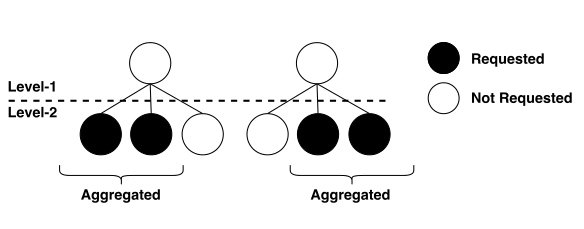
\includegraphics[scale=0.4]{Figs/tree.png}
\caption{A Practical Request Scenario in the Hierarchical Setting}
\label{fig:agg}
\end{figure}

Although the generalized scheme has a two level hierarchy (with each of the $n_1$ parallely executing instances of the basic scheme representing a node in the top level and the actual ciphertext classes representing nodes in the lower level), it avoids the pitfalls of existing hierarchical encryption based schemes \cite{akl1983cryptographic,ateniese2012provably}. In standard tree based hierarchical systems, granting access to the key corresponding to any node implicitly grants access to all the keys in the subtree rooted at that node. This means granting access to a selected set of nodes in a given subtree would blow up the key-size to be the same as the number of nodes. This is avoided in our generalized scheme, since any number of nodes (ciphertext classes) that belong to the same instance may be aggregated into a single key. Figure \ref{fig:agg} summarizes this phenomenon. In the situation depicted, a tree-based hierarchy system would require $4$ decryption keys, while our 
scheme would require only $2$. In this respect, our scheme has similar advantages to that of \cite{chu2014key}.












\section{Extending the Generalized KAC for Efficient Pairings on Elliptic Curve Subgroups}
\label{sec:extended}

The encryption schemes proposed so far use the assumption that the elliptic curve pairing bilinear pairing $\hat{e'}:\mathbb{G}_1 \times \mathbb{G}_1\longrightarrow\mathbb{G}_T$ satisfies the property $\hat{e'}(P,P) \neq 1$, where $P$ is the generator for $G_1$. In this section, we propose an extension to the generalized $n_2$-scheme that allows using pairings of the form $\hat{e''}:\mathbb{G}_1 \times \mathbb{G}_2\longrightarrow\mathbb{G}_T$, where $G_1$ and $G_2$ are two elliptic curve subgroups of the same prime order. The motivation behind this extension is that many popular pairing algorithms such as the Tate \cite{frey1994remark}, Eta \cite{hess2006eta}, and Ate \cite{zhao2008note} pairings are defined over two distinct elliptic curve subgroups $G_1$ and $G_2$ of the same order. Many efficient implementations of such pairings on sensor nodes such as TinyTate \cite{oliveira2007tinytate} have been proposed in literature. This motivates us to modify our scheme in a manner that allows using such well-known pairings. The modified encryption scheme described below allows using a pairing $\hat{e''}:\mathbb{G}_1 \times \mathbb{G}_2\longrightarrow\mathbb{G}_T$ with $P$ generator of $G_1$ and $Q$ generator of $G_2$. 


\subsection{Construction of the Extended KAC}
\label{subsec:construction}

\begin{enumerate}
 \item \textbf{Setup}$(1^{\lambda},n_2)$: Randomly pick $\alpha \in \mathbb{Z}_q$. Compute $P_i$ = ${\alpha^{i}}P \in \mathbb{G}_1$ for $i = 1,\cdots,n_2,n_2+2,\cdots,2n_2$ and $Q_i$ = ${\alpha^{i}}Q \in \mathbb{G}_2$ for $i = 1,\cdots,n_2$. Output the system parameter as\\
 $param$ = $(P,P_1,\cdots,P_{n_2},P_{n_2+2},\cdots,P_{2n_2}$,$Q,Q_1,\cdots,Q_{n_2})$. The system also randomly chooses secret parameters $t \in \mathbb{Z}_q$ which is not made public. It is only transferred through a secure channel to data owners with credentials to control client access rights.
 \item \textbf{Keygen}(): Pick $\gamma_1,\gamma_2,\cdots,\gamma_{n_1} \in \mathbb{Z}_q$, output the public and master-secret key tuple:\\ $(PK^1$=$({pk^1}_1,{pk^1}_{2},\cdots,{pk^1}_{n_1})=(\gamma_1P,\gamma_2P,\cdots,\gamma_{n_1}P)$, $PK^2$=\\$({pk^2}_1,{pk^2}_{2},\cdots,{pk^2}_{n_1})=(\gamma_1Q,\gamma_2Q,\cdots,\gamma_{n_1}Q)$, $msk$=$(\gamma_1,\gamma_2,\cdots,\gamma_{n_1}))$.
 
 \item \textbf{Encrypt}$(pk_{i_1},(i_1,i_2),m)$: For a message $m \in \mathbb{G}_T$ and an index $(i_1,i_2) \in \{1,2,\cdots,n_1\}\times\{1,2,\cdots,n_2\}$,randomly choose $r\in\mathbb{Z}_q$ and let $t'=t+r \in\mathbb{Z}_q$. Then compute the ciphertext as\\
 $\mathcal{C}$=$(rQ,t'({pk^2}_{i_1}+Q_{i_2}),m.\hat{e''}(P_{n_2},t'Q_1))$ = $(c_1,c_2,c_3)$.
 \item \textbf{Extract}$(msk=\gamma,\mathcal{S})$: For the set $\mathcal{S}$ of indices $(j_1,j_2)$ the aggregate key is computed as $K_{\mathcal{S}}$ = $(k^{1}_{\mathcal{S}},k^{2}_{\mathcal{S}},\cdots,k^{n_1}_{\mathcal{S}})$ =\\ $(\sum_{(1,j_2)\in\mathcal{S}}{\gamma_{1}}P_{n_2+1-j_2},\sum_{(2,j_2)\in\mathcal{S}}{\gamma_{2}}P_{n_2+1-j_2},\cdots,\sum_{(n_1,j_2)\in\mathcal{S}}{\gamma_{n_1}}P_{n_2+1-j_2})$\\ and the dynamic access control parameter $U$ is computed as $tQ$. Thus the net aggregate key is $(K_{\mathcal{S}},U)$ which is transmitted via a secure channel to users that have access rights to $\mathcal{S}$. Note that  $k^{j_1}_{\mathcal{S}}=\sum_{(j_1,j_2)\in\mathcal{S}}\alpha^{n+1-j_2}{pk^1}_{j_1}$ for $j_1=1,2,\cdots,n_1$. 
 \item \textbf{Decrypt}$(K_{\mathcal{S}}, U, \mathcal{S},(i_1,i_2),\mathcal{C}=\{c_1,c_2,c_3\})$: If $(i_1,i_2)\notin\mathcal{S}$, output $\bot$. Otherwise return the message\\ $\hat{m}$ = $c_3\frac{\hat{e''}(k^{i_1}_{\mathcal{S}}+\sum_{(i_1,j_2)\in\mathcal{S},j_2\neq i_2}P_{n_2+1-j_2+i_2},U+c_1)}{\hat{e''}(\sum_{(i_1,j_2)\in\mathcal{S}}P_{n_2+1-j_2},c_2)}$. 
\end{enumerate}

The proof of correctness of this scheme is presented below.

\begin{scriptsize}
\begin{equation*}
\begin{split}
 \hat{m} &= c_3\frac{\hat{e''}(k^{i_1}_{\mathcal{S}}+\sum_{(i_1,j_2)\in\mathcal{S},j_2\neq i_2}P_{n_2+1-j_2+i_2},U+c_1)}{\hat{e''}(\sum_{(i_1,j_2)\in\mathcal{S}}P_{n_2+1-j_2},c_2)}\\
%   &= c_3\frac{\hat{e''}(\sum_{(i_1,j_2)\in \mathcal{S}}{\gamma_{i_1}}P_{n_2+1-j_2} + \sum_{(i_1,j_2)\in\mathcal{S},j_2\neq i_2}P_{n_2+1-j_2+i_2},t'Q)}{\hat{e''}(\sum_{(i_1,j_2)\in\mathcal{S}}P_{n_2+1-j_2},t'({pk^2}_{i_1}+Q_{i_2}))}\\
  &= c_3\frac{\hat{e''}(\sum_{(i_1,j_2)\in \mathcal{S}}{\gamma_{i_1}}P_{n_2+1-j_2},t'Q)\hat{e''}(\sum_{(i_1,j_2)\in\mathcal{S}}(P_{n_2+1-j_2+i_2})-P_{n_2+1},t'Q)}{\hat{e''}(\sum_{(i_1,j_2)\in\mathcal{S}}P_{n_2+1-j_2},\gamma_{i_1}(t'Q))\hat{e''}(\sum_{(i_1,j_2)\in\mathcal{S}}P_{n_2+1-j_2},\alpha^{i_2}(t'Q))}\\
%   &= c_3\frac{\hat{e''}(\sum_{(i_1,j_2)\in\mathcal{S}}P_{n_2+1-j_2+i_2},t'Q)}{\hat{e''}(P_{n_2+1},t'Q)\hat{e''}(\sum_{(i_1,j_2)\in\mathcal{S}}P_{n_2+1-j_2},\alpha^{i_2}(t'Q))}\\
  &= c_3\frac{\hat{e''}(\sum_{(i_1,j_2)\in\mathcal{S}}P_{n_2+1-j_2+i_2},t'Q)}{\hat{e''}(P_{n_2+1},t'Q)\hat{e''}(\sum_{(i_1,j_2)\in\mathcal{S}}P_{n_2+1-j_2+i_2},t'Q)}\\
%   &= m\frac{\hat{e''}(P_{n_2},t'Q_1)}{\hat{e''}(P_{n_2+1},t'Q)}\\
  &= m
\end{split}  
\end{equation*}
\end{scriptsize}


\subsection{Semantic Security of the Extended KAC}
\label{subsec:proof_extended}

The proof of security uses a reduced version of the extended KAC scheme, analogous to the reduced scheme used for proving the security of the generalized KAC. The adversarial model is also the assumed to be the same as for the generalized KAC. The proof uses the $(l,l)$-BDHE assumption proposed in \ref{subsubsec:asm_2}. Let $\mathbb{G}_1$ and $\mathbb{G}_2$ be additive elliptic curve subgroups of prime order $q$, and $G_T$ be a multiplicative group of order $q$. Let $\hat{e''}:\mathbb{G}_1 \times \mathbb{G}_2\longrightarrow\mathbb{G}_T$ be a bilinear non-degenerate pairing. We claim that for any pair of positive integers $n_2,n' (n'>n_2)$ our proposed extension to the $n_2$-generalized reduced key-aggregate encryption scheme over elliptic curve subgroups is $(\tau,\epsilon,n')$ semantically secure if the decision $(\tau,\epsilon,n_2,n_2)$-BDHE assumption holds in $(\mathbb{G}_1,\mathbb{G}_2)$. We prove the claim below.

\textbf{\noindent{Proof:}} Let for a given input $n'$, $\mathcal{A}$ be a $\tau$-time adversary that has advantage greater than $\epsilon$ for the \emph{reduced scheme} parameterized with a given $n_2$. We build an algorithm $\mathcal{B}$ that has advantage at least $\epsilon$ in solving the $(n_2,n_2)$-BDHE problem in $\mathbb{G}$. Algorithm $\mathcal{B}$ takes as input a random $(n_2,n_2)$-BDHE challenge $(P,Q,H,Y_{(P,\alpha,n_2),Y'_{Q,\alpha,n_2}},Z)$ where $Z$ is either $\hat{e''}(P_{n_2+1},H)$ or a random value in $\mathbb{G}_T$. Algorithm $\mathcal{B}$ proceeds as follows.

\begin{enumerate}
 \item \textbf{Init:} Algorithm $\mathcal{B}$ runs $\mathcal{A}$ and receives the set $\mathcal{S}$ of ciphertext classes that $\mathcal{A}$ wishes to be challenged on. For each ciphertext class $(i_1,i_2)\in\mathcal{S}$, $\mathcal{B}$ performs the \textbf{SetUp}-$\mathbf{(i_1,i_2)}$, \textbf{Challenge}-$\mathbf{(i_1,i_2)}$ and \textbf{Guess}-$\mathbf{(i_1,i_2)}$ steps. Note that the number of iterations is polynomial in $|S|$. 
 
 \item \textbf{SetUp}-$\mathbf{(i_1,i_2)}$: $\mathcal{B}$ should generate the public $param$, public keys $PK^1,PK^2$, the access parameter $U$, and the aggregate key $K_{\overline{\mathcal{S}}}$. For the iteration corresponding to ciphertext class $(i_1,i_2)$, they are generated as follows.
 \begin{itemize}
  \item $param$ is set as $(P,Q,Y_{P,\alpha,n_2},Y'_{Q,\alpha,n_2})$.
  \item Randomly generate $u_1,u_2,\cdots,u_{n_1} \in \mathbb{Z}_q$. Then, set\\ $PK^1$=$({pk^1}_1,{pk^1}_2,\cdots,{pk^1}_{n_1})$, where ${pk^1}_{j_1}$ is set as $u_{j_1}P - P_{i_2}$ for $j_1=1,2,\cdots,n_1$, and set\\ $PK^2$=$({pk^2}_1,{pk^2}_2,\cdots,{pk^2}_{n_1})$, where ${pk^2}_{j_1}$ is set as $u_{j_1}Q - Q_{i_2}$ for $j_1=1,2,\cdots,n_1$
  \item $K_{\overline{\mathcal{S}}}$ is set as $(k^{1}_{\overline{\mathcal{S}}},k^{2}_{\overline{\mathcal{S}}},\cdots,k^{n_1}_{\overline{\mathcal{S}}})$ where $k^{j_1}_{\overline{\mathcal{S}}}$\\ = $\sum_{(j_1,j_2)\notin\mathcal{S}}({u_{j_1}}P_{n_2+1-j_2}-(P_{n_2+1-j_2+i_2}))$ for $j_1=1,2,\cdots,n_1$. Note that this implies $k^{j_1}_{\overline{\mathcal{S}}}$ = $\sum_{(j_1,j_2)\notin\mathcal{S}}\alpha^{n_2+1-j_2}{pk^{1}}_{j_1}$, as is supposed to be as per the scheme specification. Note that $\mathcal{B}$ knows that $(i_1,i_2)\notin \overline{\mathcal{S}}$, and hence has all the resources to compute this aggregate key for $\overline{\mathcal{S}}$. 
  \item $U$ is set as some random element in $\mathbb{G}_2$.
 \end{itemize}
 
 Note that since $P$, $Q$, $\alpha$, $U$ and the $u_{j_1}$ values are chosen uniformly at random, the public key has an identical distribution to that in the actual construction.
 
 \item \textbf{Challenge}-$\mathbf{(i_1,i_2)}$: To generate the challenge for the ciphertext class $(i_1,i_2)$, $\mathcal{B}$ computes $(c_1,c_2)$ as $(H-U,u_{i_1}H)$. It then randomly chooses a bit $b\in{(0,1)}$ and sets $K_b$ as $Z$ and $K_{1-b}$ as a random element in $\mathbb{G}_T$. The challenge given to $\mathcal{A}$ is $((c_1,c_2),K_0,K_1)$. 
 
 We claim that when $Z=\hat{e''}(P_{n_2+1},H)$ (i.e. the input to $\mathcal{B}$ is a $n_2$-BDHE tuple), then $((c_1,c_2),K_0,K_1)$ is a valid challenge to $A$. We prove this claim here. we point out that $Q$ is a generator of $\mathbb{G}_2$ and so $H=t'P$ for some $t'\in\mathbb{Z}_q$. Putting $H$ as $t'Q$ gives us the following:
 \begin{itemize}
  \item  $U=tQ$ for some $t\in\mathbb{Z}_q$
  \item $c_1=H-U=(t'-t)Q=rQ$ where $r=t'-t$
  \item $c_2=u_{i_1}H=(u_{i_1})t'Q=t'(u_{i_1}Q)=t'(u_{i_1}Q-Q_{i_2}+Q_{i_2})=t'({pk^2}_{i_1}+Q_{i_2})$
  \item $K_b=Z=\hat{e'}(P_{n_2+1},H)=\hat{e'}(P_{n_2+1},t'Q)$
 \end{itemize}
 On the other hand, if $Z$ is a random element in $\mathbb{G}_T$ (i.e. the input to $\mathcal{B}$ is a random tuple), then $K_0$ and $K_1$ are just random independent elements of $\mathbb{G}_T$.
 
 \item\textbf{Guess}-$\mathbf{(i_1,i_2)}$: The adversary $\mathcal{A}$ outputs a guess $b'$ of $b$. If $b' = b$, $\mathcal{B}$ outputs $0$ (indicating that $Z = \hat{e''}(P_{n+1},H)$), and terminates. Otherwise, it goes for the next ciphertext class in $\mathcal{S}$.
\end{enumerate}
If after $|\mathcal{S}|$ iterations, $b' \neq b$ for each ciphertext class $(i_1,i_2)\in\mathcal{S}$, the algorithm $\mathcal{B}$ outputs $1$ (indicating that $Z$ is random in $\mathbb{G}_T$). We now analyze the probability that $\mathcal{B}$ gives a correct output. If $(P,H,Y_{(P,\alpha,n_2)},Z)$ is sampled from $R'$-BDHE, $Pr[\mathcal{B}(G,H,Y_{(P,\alpha,n_2)},Z)=0]$ = $\frac{1}{2}$, while if $(P,H,Y_{(P,\alpha,n_2)},Z)$ is sampled from $L'$-BDHE, $|Pr[\mathcal{B}(G,H,Y_{(P,\alpha,n_2)},Z)]-\frac{1}{2}|$ $\geq$ $\epsilon$. So, the probability that $\mathcal{B}$ outputs correctly is at least $1-(\frac{1}{2}-\epsilon)^{|\mathcal{S}|} \geq \frac{1}{2}+\epsilon$. Thus $\mathcal{B}$ has advantage at least $\epsilon$ in solving the $(n_2,n_2)$-BDHE problem. This concludes the proof.

\section{Experimental Results Using Tate pairings}
\label{sec:results}

In this section we present experimental results from our implementations of the extended generalized scheme using Tate pairings on BN-curves using $256$ bit primes \cite{ghosh2013secure}. All our experiments have been carried out on an AMD Opteron (TM) Processor $6272\times16$ with a clock frequency $1.4$ GHz. The details of our implementations of Tate Pairings are summarized in Appendix \ref{app_sec:implementation}.

\subsection{Space and Time Complexities}

\begin{table}[!t]
\centering
\captionsetup{font=scriptsize}
\caption{Space Complexities}
\label{tab:space}
\scalebox{0.6}{
\begin{tabular}{|c|c|c|c|c|c|c|c|}
  \hline 
  $n_1$ & $n_2$ & $param$ & $PK$ & $msk$ & $K_{\mathcal{S}}$ & $U$ & Total\\
  & & (in bytes) & (in bytes) & (in bytes) & (in bytes) & (in bytes) & (in KB)\\\hline\hline
  1 & 100 & 16112 & 144 & 40 & 72 & 64 & 16.046875\\\hline
  2 & 50 & 8112 & 240 & 56 & 120 & 64 & 8.390625\\\hline
  4 & 25 & 4112 & 432 & 88 & 216 & 64 & 4.796875\\\hline
  5 & 20 & 3312 & 528 & 104 & 264 & 64 & 4.171875\\\hline
  \textbf{10} & \textbf{10} & \textbf{1712} & \textbf{1008} & \textbf{184} & \textbf{504} & \textbf{64} & \textbf{3.390625}\\\hline
  20 & 5 & 912 & 1968 & 344 & 984 & 64 & 4.171875\\\hline
  25 & 4 & 752 & 2448 & 424 & 1224 & 64 & 4.796875\\\hline
  50 & 2 & 432 & 4848 & 824 & 2424 & 64 & 8.390625\\\hline
  100 & 1 & 272 & 9648 & 1624 & 4824 & 64 & 16.046875\\\hline
  \hline
\end{tabular}}
\end{table}

\begin{table}[!t]
\centering
\captionsetup{font=scriptsize}
\caption{Time Complexities}
\label{tab:time}
\scalebox{0.6}{
% \begin{tabular}{|c|c|c|c|c|c|}
\begin{tabular}{|c|c|c|c|c|c|c|c|}
  \hline 
  $n_1$ & $n_2$ & $SetUp$ & $KeyGen$ & $Encrypt$ & $Extract$ & $Decrypt$ & Total\\
  & & (in clock cycles) & (in clock cycles) & (in clock cycles) & (in clock cycles) & (in clock cycles) & (in clock cycles)\\\hline\hline
  1 & 100 & 2920000 & 10000 & 7932000 & 47000 & 16095000 & 27004100\\\hline 
  2 & 50 & 1410000 & 30000 & 8065000 & 53000 & 16110000 & 25668000\\\hline
  4 & 25 & 690000 & 60000 & 8130000 & 81000 & 16284000 & 25245000\\\hline
  5 & 20 & 590000 & 70000 & 8091000 & 96000 & 16379000 & 25226000\\\hline
  \textbf{10} & \textbf{10} & \textbf{280000} & \textbf{140000} & \textbf{7957000} & \textbf{170000} & \textbf{16049000} & \textbf{25136000}\\\hline
  20 & 	5 & 130000 & 270000 & 8070000 & 320000 & 16361000 & 25151000\\\hline
  25 & 4 & 120000 & 350000 & 8256000 & 370000 & 16239000 & 25836000\\\hline
  50 & 2 & 50000 & 680000 & 8265000 & 712000 & 16398000 & 26105000\\\hline
  100 & 1 & 30000 & 1360000 & 8201000 & 1315000 & 16142000 & 27048000\\\hline

  \hline
\end{tabular}}
\end{table}
% \vspace{-2mm}

Table \ref{tab:space} summarizes the space requirements for various parameters of the scheme for different values of $(n_1,n_2)$. The results have been averaged over $100$ randomly chosen subsets of the $n=100$ ciphertext classes. Table \ref{tab:time} summarizes the time complexity for various operations of the scheme for different values of $(n_1,n_2)$. The results have been averaged over $100$ randomly chosen subsets of the $n=100$ ciphertext classes. The encryption and decryption operation complexities are further averaged over $10$ message transmissions corresponding to each subset. We point out that both the overall space and time requirements are minimum for $n_1=n_2=10=\surd n$, which proves the usefulnesss of the generaalization.

\subsection{Comparison with Hierarchy Based Schemes}
% \vspace{-2mm}
\begin{figure*}[!t]
\captionsetup{font=scriptsize}
\centering
% \caption{Simulation results}

% n_1:n_2	0.1	0.2	0.3	0.4	0.5	0.6	0.7	0.8	0.9
% 1:100	0.1	0.05	0.0333333	0.025	0.02	0.0166667	0.0142857	0.0125	0.0111111
% 2:50	0.2	0.1	0.0666667	0.05	0.04	0.0333333	0.0285714	0.025	0.0222222
% 4:25	0.37	0.2	0.133333	0.1	0.08	0.0666667	0.0571429	0.05	0.0497512
% 5:20	0.46	0.245	0.166667	0.125	0.1	0.0833333	0.0714286	0.0640205	0.0685871
% 10:10	0.69	0.465	0.323333	0.245	0.2	0.166667	0.150602	0.135685	0.179211
% 20:5	0.82	0.66	0.57	0.467172	0.419565	0.367647	0.34965	0.340136	0.454545
% 25:4	0.9	0.715736	0.656566	0.578534	0.5141	0.481928	0.476654	0.497018	0.617284
% 50:2	1	1	1	1	1	1	1	1	1
% 100:1	1	1	1	1	1	1	1	1	1

\begin{subfigure}{0.5\textwidth}
\captionsetup{font=scriptsize}
\centering
% \hspace*{-2.13 cm}
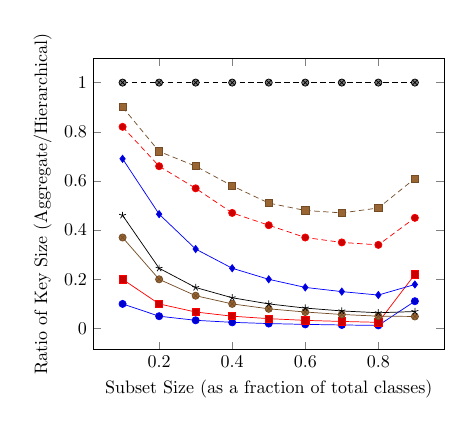
\begin{tikzpicture}[scale = 0.65]
	 \begin{axis}[
	 		xlabel=Subset Size (as a fraction of total classes),
	 		ylabel=Ratio of Key Size (Aggregate/Hierarchical),
% 	 		nolegend
	 		legend pos={north west}
	 		]
	 \addplot plot coordinates{
	 	(0.1,0.1)
		(0.2,0.05)
		(0.3,0.0333)
		(0.4,0.025)
		(0.5,0.02)
		(0.6,0.0167)
		(0.7,0.0143)
		(0.8,0.0125)
		(0.9,0.111)
	 };
	 %\addlegendentry{$n_1=1$, $n_2=100$}
	 \addplot plot coordinates{
	 	(0.1,0.2)
		(0.2,0.1)
		(0.3,0.067)
		(0.4,0.05)
		(0.5,0.04)
		(0.6,0.033)
		(0.7,0.0287)
		(0.8,0.025)
		(0.9,0.22)
	 };
	 %\addlegendentry{$n_1=2$, $n_2=50$}
	 \addplot plot coordinates{
% 	 0.37	0.2	0.133333	0.1	0.08	0.0666667	0.0571429	0.05	0.0497512
	 	(0.1,0.37)
		(0.2,0.2)
		(0.3,0.1333)
		(0.4,0.1)
		(0.5,0.08)
		(0.6,0.067)
		(0.7,0.057)
		(0.8,0.05)
		(0.9,0.049)
	 };
	 %\addlegendentry{$n_1=4$, $n_2=25$}
	 \addplot plot coordinates{
% 	 0.46	0.245	0.166667	0.125	0.1	0.0833333	0.0714286	0.0640205	0.0685871
	 	(0.1,0.46)
		(0.2,0.245)
		(0.3,0.1667)
		(0.4,0.125)
		(0.5,0.1)
		(0.6,0.083)
		(0.7,0.0714)
		(0.8,0.064)
		(0.9,0.069)
% 		(0.9,0111)
	 };
	 %\addlegendentry{$n_1=5$, $n_2=20$}
	 \addplot plot coordinates{
% 	 0.69	0.465	0.323333	0.245	0.2	0.166667	0.150602	0.135685	0.179211
	 	(0.1,0.69)
		(0.2,0.465)
		(0.3,0.323)
		(0.4,0.245)
		(0.5,0.2)
		(0.6,0.167)
		(0.7,0.150)
		(0.8,0.136)
		(0.9,0.179)
	 };
	 %\addlegendentry{$n_1=10$, $n_2=10$}
% 	 0.82	0.66	0.57	0.467172	0.419565	0.367647	0.34965	0.340136	0.454545
	 \addplot plot coordinates{
	 	(0.1,0.82)
		(0.2,0.66)
		(0.3,0.57)
		(0.4,0.47)
		(0.5,0.42)
		(0.6,0.37)
		(0.7,0.35)
		(0.8,0.34)
		(0.9,0.45)
	 };
	 %\addlegendentry{$n_1=20$, $n_2=5$}
	 \addplot plot coordinates{
% 	 0.9	0.715736	0.656566	0.578534	0.5141	0.481928	0.476654	0.497018	0.617284
	 	(0.1,0.9)
		(0.2,0.72)
		(0.3,0.66)
		(0.4,0.58)
		(0.5,0.51)
		(0.6,0.48)
		(0.7,0.47)
		(0.8,0.49)
		(0.9,0.61)
	 };
	 %\addlegendentry{$n_1=25$, $n_2=4$}
	 \addplot plot coordinates{
	 	(0.1,1)
		(0.2,1)
		(0.3,1)
		(0.4,1)
		(0.5,1)
		(0.6,1)
		(0.7,1)
		(0.8,1)
		(0.9,1)
	 };
	 %\addlegendentry{$(n_1=50$, $n_2=2)$ $\&$ $(n_1=100, n_2=1)$}
	 
	 
\end{axis}
\end{tikzpicture}
\end{subfigure}%
\begin{subfigure}{0.5\textwidth}
\captionsetup{font=scriptsize}
\centering
% \hspace*{1.13 cm}
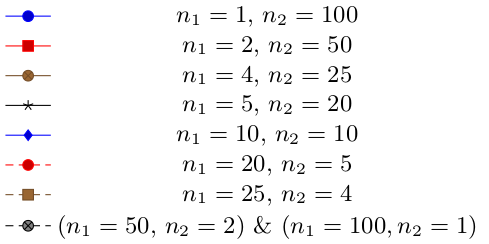
\includegraphics[scale=0.35]{Figs/Legend.png}
\end{subfigure}
\caption{Key Size ratio - Proposed Aggregate Scheme vs Hierarchical Scheme}
\label{plot:keysize}
\end{figure*}

Next, we compare specifically the key size required for the proposed extended scheme, for different values of $n_1$ and $n_2$ (again corresponding to $n=100$), with that required for a hierarchical encryption construction \cite{sandhu1988cryptographic}. Since our scheme uses a hierarchy depth of $2$, we use the same for the hierarchical construction as well, with $n_1$ nodes in level $0$, and $n_2$ level $1$ nodes in the subtree rooted at each level $0$ node. Figure \ref{plot:keysize} summarizes the findings. Evidently, lower the value of $n_1$, better the key aggregation, hence lower the ratio.

\subsection{Utilization Coefficient Comparison}
\label{subsec:util}

Finally we compare the utilization-coefficient of the extended scheme for various values of $n_1$ and $n_2$ (corresponding to $n=100$) with increase in the number of registered key pairs $l$, where each key pair increases the number of classes by $n_2$. We leave out the configuration $n_1=n,n_2=1$ because that always leads to an utilization coefficient of $1$ but is impractical due to huge space requirements. Figure \ref{fig:util} demonstrates that that beyond a certain value of $l$, the combination $(1,n)$ proposed in \cite{chu2014key} has a lower utilization coefficient that all other combinations of $(n_1,n_2)$ for a given $n$. This emphasizes the advantage of making the choice of $(n_1,n_2)$ flexible.

\begin{figure*}[!t]
\captionsetup{font=scriptsize}
\centering
\begin{subfigure}{0.5\textwidth}
\captionsetup{font=scriptsize}
\centering
% \hspace{100.13cm}
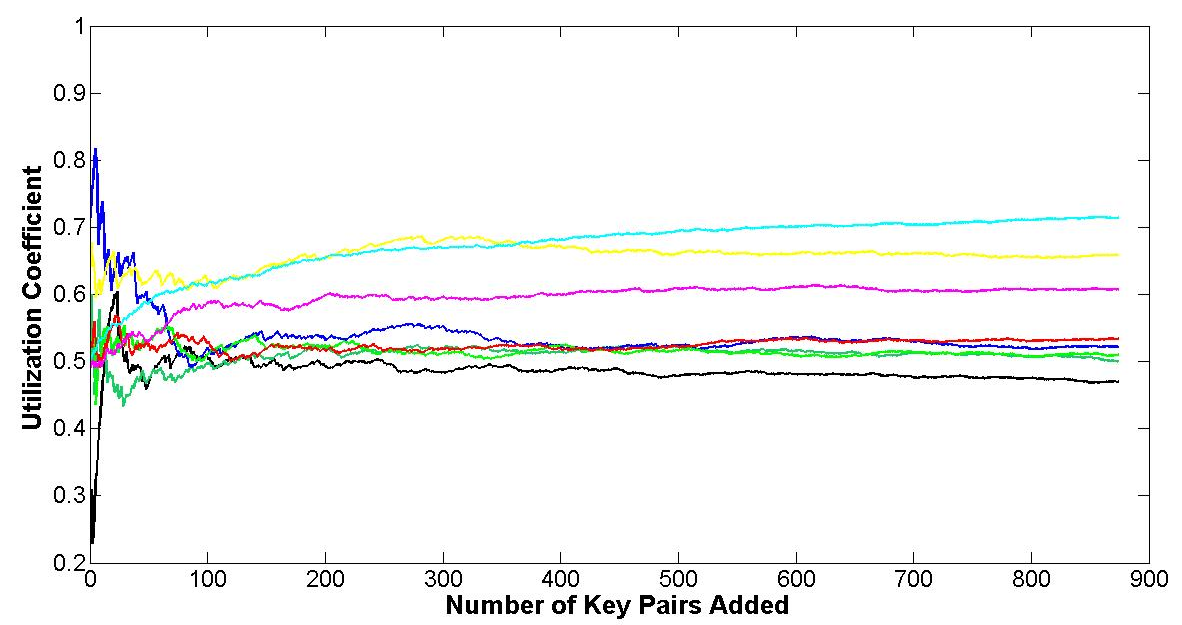
\includegraphics[scale=0.22]{Figs/UtilizationPlot.png}
\end{subfigure}%
\begin{subfigure}{0.5\textwidth}
\captionsetup{font=scriptsize}
\centering
\hspace*{3.13 cm}
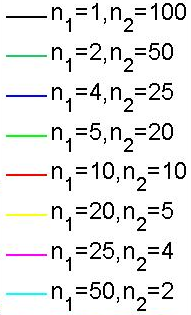
\includegraphics[scale=0.3]{Figs/Legend1.png}
\end{subfigure}
\caption{Utilization coefficient vs Newly Registered Keys}
\label{fig:util}
\end{figure*}


\section{Conclusions and Future Work}
\label{sec:conclusions}

In this paper, we have proposed a secure and dynamic key aggregate encryption scheme for online data sharing. Our scheme allows data owners to delegate users with access rights to multiple ciphertext classes using a single decryption key that combines the decrypting power of individual keys corresponding to each ciphertext class. Unlike existing key aggregate schemes that are static in their access right delegation policies, our scheme allows data owners to dynamically revoke one or more users' access rights without having to change either the public or the private parameters/keys. The use of bilinear pairings over additive elliptic curve subgroups in our scheme helps achieve massive reductions in key and ciphertext sizes over existing schemes that use multiplicative groups. We pointed out that a possible criticism of this scheme is that the number of classes is pre-defined to some fixed $n$. To deal with this issue, we next proposed a generalized two-level construction of the basic scheme that runs $n_1$ instances of the basic scheme in parallel, with each instance handling key aggregation for $n_2$ ciphertext classes. This scheme provides two major advantages. First of all, it allows dynamic extension of ciphertext classes by registering of new public key-private key pairs without affecting other system parameters. Secondly, it provides a wide range of choices for $n_1$ and $n_2$ that allows efficient utilization of ciphertext classes while also achieving optimum space and time complexities. Finally, we extend the generalized scheme to allow the use of popular and efficiently implementable bilinear pairings in literature such as Tate Pairings that operate on multiple elliptic curve subgroups instead of one. Each of the three proposed schemes have been proven to be semantically secure. Experimental studies have demonstrated the superiority of our proposed scheme over existing ones in terms of key size as well as efficient utilization of ciphertext classes. A possible future work is to make the proposed schemes secure against chosen ciphertext attacks.

\begin{scriptsize}
\bibliographystyle{unsrt}
\bibliography{bib/KeyAggregate}
\end{scriptsize}

\newpage
% \appendix


% However, KAC suffers from the following major drawbacks:
% 
% \begin{enumerate}
%  \item KAC uses bilinear non-degenerate pairings over multiplicative groups. Recent reports from NIST \cite{NIST2009} have demonstrated that the security of RSA over multiplicative cyclic groups for a key size of $1024$ bits has the same security as RSA over additive elliptic curve groups with a key size of $160$ bits. Thus defining KAC over multiplicative groups is possibly not the most computationally efficient scheme; an adaptation of the scheme to additive elliptic curve group would certainly be more efficient.
%  \item KAC is a static scheme in the sense that once a user is in possession of the aggregate key corresponding to a subset of files from data owner, the owner cannot dynamically revoke the permission of the client for accessing one or more updated files. Since dynamic changes in access rights is extremely common in shared data storage on cloud, this scenario needs to be tackled. 
%  \item The public key extension of KAC proposed in \cite{chu2014key} is extremely cumbersome and resource consuming since registration of each new public key-private key pair requires the number of classes to be extended by th original number of classes.
%  \end{enumerate}

% In this work, we aim to scheme for online data sharing that overcomes to a large extent all of the above mentioned drawbacks of KAC.

% In this paper we aim to present a scheme the above drawbacks of KAC. We also present security proofs for our proposed scheme. We then further extend the scheme using the ideas presented in \cite{} to make it secure against chosen ciphertext attacks.




\section{Bilinear Maps and the BDHE on Elliptic Curves}
\label{app_sec:prelims}

\subsection{Bilinear Pairings}

We  present a brief outline of the necessary facts about bilinear pairings on elliptic curves that are used in the forthcoming discussion. Let $\mathbb{K}=F_{p}$ be a field of prime order $p$, and let an elliptic curve over $\mathbb{K}$ be defined by the Weierstrass \cite{miller1986use} equation:
\begin{equation*}
 E(\mathbb{K}) : y^2 + a_1xy + a_3y = x^3 + a_2x^2 + a_4x + a_6
\end{equation*}

where $a_1, a_2, a_3, a_4, a_5 \in \mathbb{K}$. The curve must be non-singular. In particular, if $char(\mathbb{K})\neq2,3$, the equation takes the special form $y^2=x^3+a_4x+a_6$ with $4{a_4}^3+27{a_6}^2\neq0$. Let $\overline{K} = F_{p^k}$ be the smallest extension field of $K=F_p$ that contains the $q^{th}$ roots of unity. Here, $k$ is called the embedding degree with respect to $K$ and $q$. We denote the set of $q$-torsion points on the elliptic curve as $E(\overline{K})[q]$ ($q$-torsion points essentially have order $q$).

A pairing is a bilinear map defined over elliptic curve subgroups. Let $\mathbb{G}_{1}$ and $\mathbb{G}_{2}$ be two such additive cyclic subgroups of the same prime order $q$ and let $\mathbb{G}_{T}$ be a multiplicative group, also of order $q$ with identity element $1$. Let $P$ and $Q$ be generators for $\mathbb{G}_1$ and $\mathbb{G}_2$ respectively. A pairing $\hat{e'}:\mathbb{G}_1 \times \mathbb{G}_2\longrightarrow\mathbb{G}_T$ satisfying the following the following properties is said to be a bilinear mapping. 

\begin{itemize}
 \item Bilinear: $\forall P_1,P_2 \in \mathbb{G}_1, Q_1,Q_2\in\mathbb{G}_2$, and $a,b \in \mathbb{Z}$, we have the following:
 \begin{eqnarray}
   \hat{e'}(aP_1,bQ_1) &= \hat{e'}(P_1,Q_1)^{ab}\nonumber\\
   \hat{e'}(P_1+P_2,Q_1) &= \hat{e'}(P_1,Q_1)\hat{e'}(P_2,Q_1)\nonumber\\
   \hat{e'}(P_1,Q_1+Q_2) &= \hat{e'}(P_1,Q_1)\hat{e'}(P_1,Q_2)\nonumber
 \end{eqnarray}
 \item Non-degeneracy: If for all $P_i \in \mathbb{G}_1, \hat{e'}(P_1,Q_1)=1$ then $Q_1=\mathcal{0}$. Alternatively, if $P$ and $Q$ be the generators for $\mathbb{G}_1$ and $\mathbb{G}_2$ respectively where neither group only contains the point at infinity, then $\hat{e'}(P,Q)\neq1$ 
 \item Computability: There exists an efficient algorithm to compute $\hat{e'}(R,S)\forall R \in \mathbb{G}_1, S\in\mathbb{G}_2$
\end{itemize}

It is important to note that $\mathbb{G}_1$ and $\mathbb{G}_2$ could be identical groups as well.

% \subsection{The Decisional Bilinear Diffie-Hellman Problem (DBDH)}

% The three-party Diffie-Hellman key agreement \cite{} lends itself to the decisional form - the decisional bilinear Diffie-Hellman (DBDH) problem. DBDH requires a participant to determine if some target element is either a special combination of given parameters or a random element

% Let $\mathbb{G}$ be an additive cyclic elliptic curve subgroup of prime order $q$, where $2^{\lambda}\leq q \leq 2^{\lambda + 1}$, such that the point $P$ is a generator for $\mathbb{G}$. Also, let $\mathbb{G}_{T}$ be a multiplicative group of order $q$ with identity element $1$. We assume that there exists an efficiently computable bilinear pairing $\hat{e'}:\mathbb{G} \times \mathbb{G}\longrightarrow\mathbb{G}_T$. The DBDH problem is defined as follows.  Given $aP, bP, cP \in \mathbb{G}$ where $a,b,c\in \mathbb{Z}_q$, and $T\in \mathbb{G}_T$, determine if $T=\hat{e'}(P,P)^{abc}$. 

% \subsection{The Bilinear Diffie-Hellman Exponent Problem (BDHE)}







\section{Semantic Security of Key-Aggregate Schemes}
\label{app_sec:security}

We now define the semantic security of a key-aggregate encryption system against an adversary using the following game between an attack algorithm $\mathcal{A}$ and a challenger $\mathcal{B}$. Both $\mathcal{A}$ and $\mathcal{B}$ are given $n$, the total number of ciphertext classes, as input. The game proceeds through the following stages.

\begin{enumerate}
 \item \textbf{Init:} Algorithm $\mathcal{A}$ begins by outputting a set $\mathcal{S} \subset \{1,2,\cdots,n\}$ of receivers that it wants to
attack.  For each ciphertext class $i\in\mathcal{S}$, challenger $\mathcal{B}$ performs the \textbf{SetUp}-$\mathbf{i}$, \textbf{Challenge}-$\mathbf{i}$ and \textbf{Guess}-$\mathbf{i}$ steps. Note that the number of iterations is polynomial in $|S|$.

 \item \textbf{SetUp}-$\mathbf{i}$: Challenger $\mathcal{B}$ generates the public $param$, public key $PK$, the access parameter $U$, and provides them to $\mathcal{A}$. In addition, $\mathcal{B}$ also generates and furnishes $\mathcal{A}$ with the aggregate key $K_{\overline{\mathcal{S}}}$ that allows $\mathcal{A}$ to decrypt any ciphertext class $j\notin\mathcal{S}$. 
 \item \textbf{Challenge}-$\mathbf{i}$: Challenger $\mathcal{B}$ performs an encryption of the secret message $m_i$ belonging to the $i^{th}$ class to obtain the ciphertext $\mathcal{C}$. Next, $\mathcal{B}$ picks a random $b\in{(0,1)}$. It sets $T_b = m_i$ and picks a random $T_{1- b}$ from the set of possible plaintext messages. It then gives $(\mathcal{C}, T_0, T_1)$ to algorithm $\mathcal{A}$ as a challenge.

 
 \item\textbf{Guess}-$\mathbf{i}$: The adversary $\mathcal{A}$ outputs a guess $b'$ of $b$. If $b' = b$, $\mathcal{A}$ wins. Otherwise, the game moves on to the next ciphertext class in $\mathcal{S}$ until all ciphertext classes in $\mathcal{S}$ are exhausted.
\end{enumerate}
% \vspace{-2mm}
If $\mathcal{A}$ fails to predict correctly for all ciphertext classes in $\mathcal{S}$, then $\mathcal{A}$ loses the game. Let $AdvKAC_{\mathcal{A},n}$ denote the probability that $\mathcal{A}$ wins the game when the challenger is given $n$ as input. We say that a key-aggregate encryption system is $(\tau,\epsilon,n)$ semantically secure if for all $\tau$-time algorithms $\mathcal{A}$ we have that $|AdvKAC_{\mathcal{A},n}-\frac{1}{2}| < \epsilon$ where $\epsilon$ is a very small quantity. 

The above mentioned game could be looked upon as analogous to a practical attack scenario where users with decryption rights to ciphertext classes not in $\mathcal{S}$, launch a combined attack on $\mathcal{S}$. The adversary $\mathcal{A}$ chooses the subset $\mathcal{S}$ of ciphertext classes she wishes to attack. Note that the adversary $\mathcal{A}$ is non-adaptive; it chooses $\mathcal{S}$, and obtains the aggregate decryption key for all ciphertext classes outside of $\mathcal{S}$, before it even sees the public parameters $param$ or the public key $PK$. An adaptive adversary could request ciphertext classes adaptively. We prove the security of our proposed schemes in the non-adaptive settings described above. We also note that our definition of semantic security for key-aggregate cryptosystems is similar to that for broadcast encryption systems proposed in \cite{boneh2005collusion}.

 

\section{Proof of Correctness of the Generalized Key-Aggregate Encryption Scheme}
\label{app_sec:correct_general}

In this section, we present a proof of correctness for the generalized key-aggregate encryption scheme. Let $\hat{m}$ be the output message produced by decryption corresponding to the plaintext $m$. We assume that the output is not $\bot$. 

\begin{scriptsize}
\begin{equation}
\begin{split}
 \hat{m} &= c_3\frac{\hat{e'}(k^{i_1}_{\mathcal{S}}+\sum_{(i_1,j_2)\in\mathcal{S},j_2\neq i_2}P_{n_2+1-j_2+i_2},U+c_1)}{\hat{e'}(\sum_{(i_1,j_2)\in\mathcal{S}}P_{n_2+1-j_2},c_2)}\\
  &= c_3\frac{\hat{e'}(\sum_{(i_1,j_2)\in \mathcal{S}}{\gamma_{i_1}}P_{n_2+1-j_2} + \sum_{(i_1,j_2)\in\mathcal{S},j_2\neq i_2}P_{n_2+1-j_2+i_2},t'P)}{\hat{e'}(\sum_{(i_1,j_2)\in\mathcal{S}}P_{n_2+1-j_2},t'(pk_{i_1}+P_{i_2})}\\
  &= c_3\frac{\hat{e'}(\sum_{(i_1,j_2)\in \mathcal{S}}{\gamma_{i_1}}P_{n_2+1-j_2},t'P)\hat{e'}(\sum_{(i_1,j_2)\in\mathcal{S}}(P_{n_2+1-j_2+i_2})-P_{n_2+1},t'P)}{\hat{e'}(\sum_{(i_1,j_2)\in\mathcal{S}}P_{n_2+1-j_2},t'pk_{i_1})\hat{e'}(\sum_{(i_1,j_2)\in\mathcal{S}}P_{n_2+1-j_2},t'P_{i_2})}\\
  &= c_3\frac{\hat{e'}(\sum_{(i_1,j_2)\in\mathcal{S}}P_{n_2+1-j_2+i_2},t'P)}{\hat{e'}(P_{n_2+1},t'P)\hat{e'}(\sum_{(i_1,j_2)\in\mathcal{S}}P_{n_2+1-j_2},t'P_{i_2})}\\
  &= c_3\frac{\hat{e'}(\sum_{(i_1,j_2)\in\mathcal{S}}P_{n_2+1-j_2+i_2},t'P)}{\hat{e'}(P_{n_2+1},t'P)\hat{e'}(\sum_{(i_1,j_2)\in\mathcal{S}}P_{n_2+1-j_2+i_2},t'P)}\\
  &= m\frac{\hat{e'}(P_{n_2},t'P_1)}{\hat{e'}(P_{n_2+1},t'P)}\\
  &= m
\end{split}  
\end{equation}
\end{scriptsize}


\section{Proof of Semantic Security of the Generalized Key-Aggregate Encryption Scheme}
\label{app_sec:proof_general}

\subsection{The Reduced Generalized Scheme}

As in the original scheme, we may analogously define a reduced version of the generalized encryption scheme. We note that once again, in the generalized scheme, the ciphertext $\mathcal{C}=(c_1,c_2,c_3)$ output by the $Encypt$ operation essentially embeds the value of $m$ in $c_3$ by multiplying it with $\hat{e'}(P_{n_2},tP_1)$. Consequently, the security of our proposed scheme is equivalent to that of a \emph{reduced} generalized key-aggregate encryption scheme that simply uses the reduced ciphertext $(c_1,c_2)$, the aggregate key $K_{\mathcal{S}}$ and the dynamic access parameter $U$ to successfully transmit and decrypt the value of $\hat{e'}(P_{n_2},t'P_1)=\hat{e'}(P_{n_2+1},t'P)$. We prove the semantic security of this \emph{reduced scheme} parameterized with a given number of ciphertext classes $n_2$ for each instance, which also amounts to proving the semantic security of our original encryption scheme for the same number of ciphertext classes. Note that the proof of security is independent of the 
number of instances $n_1$ that run in parallel.

\subsection{The Adversarial Model} We make the following assumptions about the adversary $\mathcal{A}$:

\begin{enumerate}
 \item The adversary has the aggregate key that allows her to access any ciphertext class other than those in the target subset $\mathcal{S}$, that is, she possesses $K_{\overline{\mathcal{S}}}$.
 \item The adversary has access to the public parameters $param$ and $PK$, and also possesses the dynamic access parameter $U$.
%  \item The adversary is authorized and and hence 
\end{enumerate}


\subsection{The Security Proof}

The security proof presented here uses the first complexity assumption stated in \ref{subsubsec:asm_1}. Let $\mathbb{G}$ be a bilinear elliptic curve subgroup of prime order $q$ and $G_T$ be a multiplicative group of order $q$. Let $\hat{e'}:\mathbb{G} \times \mathbb{G}\longrightarrow\mathbb{G}_T$ be a bilinear non-degenerate pairing. For any pair of positive integers $n_2,n' (n'>n_2)$ our proposed $n_2$-generalized reduced key-aggregate encryption scheme over elliptic curve subgroups is $(\tau,\epsilon,n')$ semantically secure if the decision $(\tau,\epsilon,n_2)$-BDHE assumption holds in $\mathbb{G}$. We now prove this statement below.

\textbf{\noindent{Proof:}} Let for a given input $n'$, $\mathcal{A}$ be a $\tau$-time adversary that has advantage greater than $\epsilon$ for the \emph{reduced scheme} parameterized with a given $n_2$. We build an algorithm $\mathcal{B}$ that has advantage at least $\epsilon$ in solving the $n_2$-BDHE problem in $\mathbb{G}$. Algorithm $\mathcal{B}$ takes as input a random $n_2$-BDHE challenge $(P,H,Y_{(P,\alpha,n_2)},Z)$ where $Z$ is either $\hat{e'}(P_{n_2+1},H)$ or a random value in $\mathbb{G}_T$. Algorithm $\mathcal{B}$ proceeds as follows.

\begin{enumerate}
 \item \textbf{Init:} Algorithm $\mathcal{B}$ runs $\mathcal{A}$ and receives the set $\mathcal{S}$ of ciphertext classes that $\mathcal{A}$ wishes to be challenged on. For each ciphertext class $(i_1,i_2)\in\mathcal{S}$, $\mathcal{B}$ performs the \textbf{SetUp}-$\mathbf{(i_1,i_2)}$, \textbf{Challenge}-$\mathbf{(i_1,i_2)}$ and \textbf{Guess}-$\mathbf{(i_1,i_2)}$ steps. Note that the number of iterations is polynomial in $|S|$. 
 
 \item \textbf{SetUp}-$\mathbf{(i_1,i_2)}$: $\mathcal{B}$ should generate the public $param$, public key $PK$, the access parameter $U$, and the aggregate key $K_{\overline{\mathcal{S}}}$. For the iteration corresponding to ciphertext class $(i_1,i_2)$, they are generated as follows.
 \begin{itemize}
  \item $param$ is set as $(P,Y_{P,\alpha,n_2})$.
  \item Randomly generate $u_1,u_2,\cdots,u_{n_1} \in \mathbb{Z}_q$. Then, set\\ $PK$=$(pk_1,pk_2,\cdots,pk_{n_1})$, where $pk_{j_1}$ is set as $u_{j_1}P - P_{i_2}$ for $j_1=1,2,\cdots,n_1$.
  \item $K_{\overline{\mathcal{S}}}$ is set as $(k^{1}_{\overline{\mathcal{S}}},k^{2}_{\overline{\mathcal{S}}},\cdots,k^{n_1}_{\overline{\mathcal{S}}})$ where $k^{j_1}_{\overline{\mathcal{S}}}$ = $\sum_{(j_1,j_2)\notin\mathcal{S}}({u}P_{n_2+1-j_2}-(P_{n_2+1-j_2+i_2}))$ for $j_1=1,2,\cdots,n_1$. Note that this implies $k^{j_1}_{\overline{\mathcal{S}}}$ is equal to $\sum_{(j_1,j_2)\notin\mathcal{S}}\alpha^{n_2+1-j_2}pk_{j_1}$, as is supposed to be as per the scheme specification. Note that $\mathcal{B}$ knows that $(i_1,i_2)\notin \overline{\mathcal{S}}$, and hence has all the resources to compute this aggregate key for $\overline{\mathcal{S}}$. 
  \item $U$ is set as some random element in $\mathbb{G}$.
 \end{itemize}
 
 Note that since $P$, $\alpha$, $U$ and the $u_{j_1}$ values are chosen uniformly at random, the public key has an identical distribution to that in the actual construction.
 
 \item \textbf{Challenge}-$\mathbf{(i_1,i_2)}$: To generate the challenge for the ciphertext class $(i_1,i_2)$, $\mathcal{B}$ computes $(c_1,c_2)$ as $(H-U,u_{i_1}H)$. It then randomly chooses a bit $b\in{(0,1)}$ and sets $T_b$ as $Z$ and $T_{1-b}$ as a random element in $\mathbb{G}_T$. The challenge given to $\mathcal{A}$ is $((c_1,c_2),T_0,T_1)$. 
 
 We claim that when $Z=\hat{e'}(P_{n_2+1},H)$ (i.e. the input to $\mathcal{B}$ is a $n_2$-BDHE tuple), then $((c_1,c_2),T_0,T_1)$ is a valid challenge to $A$. We prove this claim here. we point out that $P$ is a generator of $\mathbb{G}$ and so $H=t'P$ for some $t'\in\mathbb{Z}_q$. Putting $H$ as $t'P$ gives us the following:
 \begin{itemize}
  \item  $U=tP$ for some $t\in\mathbb{Z}_q$
  \item $c_1=H-U=(t'-t)P=rP$ for $r=t'-t$
  \item $c_2=u_{i_1}H=(u_{i_1})t'P=t'(u_{i_1}P)=t'(u_{i_1}P-P_{i_2}+P_{i_2})=t'(pk_{i_1}+P_{i_2})$
  \item $K_b=Z=\hat{e'}(P_{n_2+1},H)=\hat{e'}(P_{n_2+1},t'P)$
 \end{itemize}
 On the other hand, if $Z$ is a random element in $\mathbb{G}_T$ (i.e. the input to $\mathcal{B}$ is a random tuple), then $K_0$ and $K_1$ are just random independent elements of $\mathbb{G}_T$.
 
 \item\textbf{Guess}-$\mathbf{(i_1,i_2)}$: The adversary $\mathcal{A}$ outputs a guess $b'$ of $b$. If $b' = b$, $\mathcal{B}$ outputs $0$ (indicating that $Z = \hat{e'}(P_{n+1},H)$), and terminates. Otherwise, it goes for the next ciphertext class in $\mathcal{S}$.
\end{enumerate}
If after $|\mathcal{S}|$ iterations, $b' \neq b$ for each ciphertext class $(i_1,i_2)\in\mathcal{S}$, the algorithm $\mathcal{B}$ outputs $0$ (indicating that $Z = \hat{e'}(P_{n_2+1},H)$). Otherwise, it outputs $1$ (indicating that $Z$ is random in $\mathbb{G}_T$). We now analyze the probability that $\mathcal{B}$ gives a correct output. If $(P,H,Y_{(P,\alpha,n_2)},Z)$ is sampled from $R$-BDHE, $Pr[\mathcal{B}(G,H,Y_{(P,\alpha,n_2)},Z)=0]$ = $\frac{1}{2}$, while if $(P,H,Y_{(P,\alpha,n_2)},Z)$ is sampled from $L$-BDHE, $|Pr[\mathcal{B}(G,H,Y_{(P,\alpha,n_2)},Z)]-\frac{1}{2}|$ $\geq$ $\epsilon$. So, the probability that $\mathcal{B}$ outputs correctly is at least $1-(\frac{1}{2}-\epsilon)^{|\mathcal{S}|} \geq \frac{1}{2}+\epsilon$. Thus $\mathcal{B}$ has advantage at least $\epsilon$ in solving the $n_2$-BDHE problem. This concludes the proof.


\section{Proof of Correctness of the Extended Key-Aggregate Encryption Scheme:}
\label{app_sec:correct_extended}

In this section, we present a proof of correctness for the extended key-aggregate encryption scheme. Let $\hat{m}$ be the output message produced by decryption corresponding to the plaintext $m$. We assume that the output is not $\bot$. 

\begin{scriptsize}
\begin{equation}
\begin{split}
 \hat{m} &= c_3\frac{\hat{e''}(k^{i_1}_{\mathcal{S}}+\sum_{(i_1,j_2)\in\mathcal{S},j_2\neq i_2}P_{n_2+1-j_2+i_2},U+c_1)}{\hat{e''}(\sum_{(i_1,j_2)\in\mathcal{S}}P_{n_2+1-j_2},c_2)}\\
  &= c_3\frac{\hat{e''}(\sum_{(i_1,j_2)\in \mathcal{S}}{\gamma_{i_1}}P_{n_2+1-j_2} + \sum_{(i_1,j_2)\in\mathcal{S},j_2\neq i_2}P_{n_2+1-j_2+i_2},t'Q)}{\hat{e''}(\sum_{(i_1,j_2)\in\mathcal{S}}P_{n_2+1-j_2},t'({pk^2}_{i_1}+Q_{i_2}))}\\
  &= c_3\frac{\hat{e''}(\sum_{(i_1,j_2)\in \mathcal{S}}{\gamma_{i_1}}P_{n_2+1-j_2},t'Q)\hat{e''}(\sum_{(i_1,j_2)\in\mathcal{S}}(P_{n_2+1-j_2+i_2})-P_{n_2+1},t'Q)}{\hat{e''}(\sum_{(i_1,j_2)\in\mathcal{S}}P_{n_2+1-j_2},\gamma_{i_1}(t'Q))\hat{e''}(\sum_{(i_1,j_2)\in\mathcal{S}}P_{n_2+1-j_2},\alpha^{i_2}(t'Q))}\\
  &= c_3\frac{\hat{e''}(\sum_{(i_1,j_2)\in\mathcal{S}}P_{n_2+1-j_2+i_2},t'Q)}{\hat{e''}(P_{n_2+1},t'Q)\hat{e''}(\sum_{(i_1,j_2)\in\mathcal{S}}P_{n_2+1-j_2},\alpha^{i_2}(t'Q))}\\
  &= c_3\frac{\hat{e''}(\sum_{(i_1,j_2)\in\mathcal{S}}P_{n_2+1-j_2+i_2},t'Q)}{\hat{e''}(P_{n_2+1},t'Q)\hat{e''}(\sum_{(i_1,j_2)\in\mathcal{S}}P_{n_2+1-j_2+i_2},t'Q)}\\
  &= m\frac{\hat{e''}(P_{n_2},t'Q_1)}{\hat{e''}(P_{n_2+1},t'Q)}\\
  &= m
\end{split}  
\end{equation}
\end{scriptsize}

\section{Proof of Semantic Security of the Extended Key-Aggregate Encryption Scheme}
\label{app_sec:proof_extended}

\subsection{The Reduced Version of the Extended Key-Aggregate Scheme}

As in the earlier schemes, we define a reduced version of the extension to the generalized encryption scheme. The security of our proposed extended scheme is equivalent to that of a \emph{reduced} scheme that simply uses the reduced ciphertext $(c_1,c_2)$, the aggregate key $K_{\mathcal{S}}$ and the dynamic access parameter $U$ to successfully transmit and decrypt the value of $\hat{e'}(P_{n_2},t'Q_1)=\hat{e'}(P_{n_2+1},t'Q)$. We prove the semantic security of this \emph{reduced scheme} parameterized with a given number of ciphertext classes $n_2$ for each instance, which also amounts to proving the semantic security of our original encryption scheme for the same number of ciphertext classes. Note that the proof of security is independent of the number of instances $n_1$ that run in parallel.

\subsection{The Adversarial Model} We make the following assumptions about the adversary $\mathcal{A}$:

\begin{enumerate}
 \item The adversary has the aggregate key that allows her to access any ciphertext class other than those in the target subset $\mathcal{S}$, that is, she possesses $K_{\overline{\mathcal{S}}}$.
 \item The adversary has access to the public parameters $param$, $PK^1$ and $PK^2$, and also possesses the dynamic access parameter $U$.
%  \item The adversary is authorized and and hence 
\end{enumerate}


\subsection{The Security Proof}

The security proof presented here uses the second complexity assumption stated in \ref{subsubsec:asm_2}. Let $\mathbb{G_1}$ and $\mathbb{G}_2$ be additive elliptic curve subgroups of prime order $q$, and $G_T$ be a multiplicative group of order $q$. Let $\hat{e''}:\mathbb{G}_1 \times \mathbb{G}_2\longrightarrow\mathbb{G}_T$ be a bilinear non-degenerate pairing. We claim that for any pair of positive integers $n_2,n' (n'>n_2)$ our proposed extension to the $n_2$-generalized reduced key-aggregate encryption scheme over elliptic curve subgroups is $(\tau,\epsilon,n')$ semantically secure if the decision $(\tau,\epsilon,n_2,n_2)$-BDHE assumption holds in $(\mathbb{G}_1,\mathbb{G}_2)$. \textbf{As already proved in Appendix \ref{app_sec:hardness}, the decision $(\tau,\epsilon,l,l)$-BDHE assumption for elliptic curves holds in equi-prime order subgroups $(\mathbb{G}_1,\mathbb{G}_2)$ if the decision $(\tau,\epsilon,l)$-BDHE assumption for elliptic curves holds in $\mathbb{G}_1$}. Thus proving the aforementioned 
claim amounts to proving that our proposed extension to the $n_2$-generalized reduced key-aggregate encryption scheme over elliptic curve subgroups is $(\tau,\epsilon,n')$ semantically secure if the decision $(\tau,\epsilon,l)$-BDHE assumption for elliptic curves holds in $\mathbb{G}_1$. We now prove the claim below.

\textbf{\noindent{Proof:}} Let for a given input $n'$, $\mathcal{A}$ be a $\tau$-time adversary that has advantage greater than $\epsilon$ for the \emph{reduced scheme} parameterized with a given $n_2$. We build an algorithm $\mathcal{B}$ that has advantage at least $\epsilon$ in solving the $(n_2,n_2)$-BDHE problem in $\mathbb{G}$. Algorithm $\mathcal{B}$ takes as input a random $(n_2,n_2)$-BDHE challenge $(P,Q,H,Y_{(P,\alpha,n_2),Y'_{Q,\alpha,n_2}},Z)$ where $Z$ is either $\hat{e''}(P_{n_2+1},H)$ or a random value in $\mathbb{G}_T$. Algorithm $\mathcal{B}$ proceeds as follows.

\begin{enumerate}
 \item \textbf{Init:} Algorithm $\mathcal{B}$ runs $\mathcal{A}$ and receives the set $\mathcal{S}$ of ciphertext classes that $\mathcal{A}$ wishes to be challenged on. For each ciphertext class $(i_1,i_2)\in\mathcal{S}$, $\mathcal{B}$ performs the \textbf{SetUp}-$\mathbf{(i_1,i_2)}$, \textbf{Challenge}-$\mathbf{(i_1,i_2)}$ and \textbf{Guess}-$\mathbf{(i_1,i_2)}$ steps. Note that the number of iterations is polynomial in $|S|$. 
 
 \item \textbf{SetUp}-$\mathbf{(i_1,i_2)}$: $\mathcal{B}$ should generate the public $param$, public keys $PK^1,PK^2$, the access parameter $U$, and the aggregate key $K_{\overline{\mathcal{S}}}$. For the iteration corresponding to ciphertext class $(i_1,i_2)$, they are generated as follows.
 \begin{itemize}
  \item $param$ is set as $(P,Q,Y_{P,\alpha,n_2},Y'_{Q,\alpha,n_2})$.
  \item Randomly generate $u_1,u_2,\cdots,u_{n_1} \in \mathbb{Z}_q$. Then, set\\ $PK^1$=$({pk^1}_1,{pk^1}_2,\cdots,{pk^1}_{n_1})$, where ${pk^1}_{j_1}$ is set as $u_{j_1}P - P_{i_2}$ for $j_1=1,2,\cdots,n_1$, and set\\ $PK^2$=$({pk^2}_1,{pk^2}_2,\cdots,{pk^2}_{n_1})$, where ${pk^2}_{j_1}$ is set as $u_{j_1}Q - Q_{i_2}$ for $j_1=1,2,\cdots,n_1$
  \item $K_{\overline{\mathcal{S}}}$ is set as $(k^{1}_{\overline{\mathcal{S}}},k^{2}_{\overline{\mathcal{S}}},\cdots,k^{n_1}_{\overline{\mathcal{S}}})$ where $k^{j_1}_{\overline{\mathcal{S}}}$ = $\sum_{(j_1,j_2)\notin\mathcal{S}}({u}P_{n_2+1-j_2}-(P_{n_2+1-j_2+i_2}))$ for $j_1=1,2,\cdots,n_1$. Note that this implies $k^{j_1}_{\overline{\mathcal{S}}}$ is equal to $\sum_{(j_1,j_2)\notin\mathcal{S}}\alpha^{n_2+1-j_2}{pk^{1}}_{j_1}$, as is supposed to be as per the scheme specification. Note that $\mathcal{B}$ knows that $(i_1,i_2)\notin \overline{\mathcal{S}}$, and hence has all the resources to compute this aggregate key for $\overline{\mathcal{S}}$. 
  \item $U$ is set as some random element in $\mathbb{G}_2$.
 \end{itemize}
 
 Note that since $P$, $Q$, $\alpha$, $U$ and the $u_{j_1}$ values are chosen uniformly at random, the public key has an identical distribution to that in the actual construction.
 
 \item \textbf{Challenge}-$\mathbf{(i_1,i_2)}$: To generate the challenge for the ciphertext class $(i_1,i_2)$, $\mathcal{B}$ computes $(c_1,c_2)$ as $(H-U,u_{i_1}H)$. It then randomly chooses a bit $b\in{(0,1)}$ and sets $T_b$ as $Z$ and $T_{1-b}$ as a random element in $\mathbb{G}_T$. The challenge given to $\mathcal{A}$ is $((c_1,c_2),T_0,T_1)$. 
 
 We claim that when $Z=\hat{e''}(P_{n_2+1},H)$ (i.e. the input to $\mathcal{B}$ is a $n_2$-BDHE tuple), then $((c_1,c_2),T_0,T_1)$ is a valid challenge to $A$. We prove this claim here. we point out that $Q$ is a generator of $\mathbb{G}_2$ and so $H=t'P$ for some $t'\in\mathbb{Z}_q$. Putting $H$ as $t'Q$ gives us the following:
 \begin{itemize}
  \item  $U=tQ$ for some $t\in\mathbb{Z}_q$
  \item $c_1=H-U=(t'-t)Q=rQ$ where $r=t'-t$
  \item $c_2=u_{i_1}H=(u_{i_1})t'Q=t'(u_{i_1}Q)=t'(u_{i_1}Q-Q_{i_2}+Q_{i_2})=t'({pk^2}_{i_1}+Q_{i_2})$
  \item $K_b=Z=\hat{e'}(P_{n_2+1},H)=\hat{e'}(P_{n_2+1},t'Q)$
 \end{itemize}
 On the other hand, if $Z$ is a random element in $\mathbb{G}_T$ (i.e. the input to $\mathcal{B}$ is a random tuple), then $K_0$ and $K_1$ are just random independent elements of $\mathbb{G}_T$.
 
 \item\textbf{Guess}-$\mathbf{(i_1,i_2)}$: The adversary $\mathcal{A}$ outputs a guess $b'$ of $b$. If $b' = b$, $\mathcal{B}$ outputs $0$ (indicating that $Z = \hat{e''}(P_{n+1},H)$), and terminates. Otherwise, it goes for the next ciphertext class in $\mathcal{S}$.
\end{enumerate}
If after $|\mathcal{S}|$ iterations, $b' \neq b$ for each ciphertext class $(i_1,i_2)\in\mathcal{S}$, the algorithm $\mathcal{B}$ outputs $0$ (indicating that $Z = \hat{e'}(P_{n_2+1},H)$). Otherwise, it outputs $1$ (indicating that $Z$ is random in $\mathbb{G}_T$). We now analyze the probability that $\mathcal{B}$ gives a correct output. If $(P,H,Y_{(P,\alpha,n_2)},Z)$ is sampled from $R'$-BDHE, $Pr[\mathcal{B}(G,H,Y_{(P,\alpha,n_2)},Z)=0]$ = $\frac{1}{2}$, while if $(P,H,Y_{(P,\alpha,n_2)},Z)$ is sampled from $L'$-BDHE, $|Pr[\mathcal{B}(G,H,Y_{(P,\alpha,n_2)},Z)]-\frac{1}{2}|$ $\geq$ $\epsilon$. So, the probability that $\mathcal{B}$ outputs correctly is at least $1-(\frac{1}{2}-\epsilon)^{|\mathcal{S}|} \geq \frac{1}{2}+\epsilon$. Thus $\mathcal{B}$ has advantage at least $\epsilon$ in solving the $(n_2,n_2)$-BDHE problem. This concludes the proof.

\section{Implementation of Tate pairings Using BN Curves}
\label{app_sec:implementation}

\subsection{The Tate pairing}
% \label{app_subsec:tate}

We first provide a brief overview of the Tate pairing. Let $\mathbb{K}$ be a field of prime order $p$, and let an elliptic curve $E(K)$ over $\mathbb{K}$ be defined by the Weierstrass \cite{miller1986use} equation. Also, Let $\overline{K} = F_{p^k}$ be the smallest extension field of $K=F_p$ that contains the $q^{th}$ roots of unity. We refer to $k$ as the embedding degree with respect to $K$ and $q$. Further, we refer to the set of $q$-torsion points on the elliptic curve as $E(\overline{K})[q]$ ($q$-torsion points essentially have order $q$). Before defining the Tate pairing, we briefly state the Miller's function \cite{miller1986use}. Let $[a]P$ denote the multiplication of a point $P \in E$ by a scalar $a \in \mathbb{Z}$ (equivalent to adding $P$ $a$ times), and let $\mathcal{O} \in E$ denote the point at infinity. A Miller function is any rational function on $E$ that has a divisor of the form
  \begin{equation}
   (f_{q,P}) = q(P)-([q]P)-(q-1)\mathcal{O}.
  \end{equation}
A Miller function has $q$ zeros at $P$, one pole at $[q]P$ and $q-1$ poles at $\mathcal{O}$. For every point $Q\neq P, [q]P, \mathcal{0}$, we have $(f_{q,P})\in {\overline{K}}^{*}$. We now define the Tate pairing over elliptic curves. 

The Tate pairing $e_{T}:\mathbb{G}_1\times \mathbb{G}_2\longrightarrow \mathbb{G}_T$ is a well-defined, non-degenerate, bilinear pairing with $\mathbb{G}_1 = E(K)[q]$, $\mathbb{G}_2=E(\overline{K})/qE(\overline{K})$, and $\mathbb{G}_T = {\overline{K}}^*/({\overline{K}}^{*})^q$. Let $P \in E(\overline{K})[q]$ and $Q \in E(\overline{K})/qE(\overline{K})$. Then the Tate pairing of $P,Q$ is computed as 
\begin{equation}
 e_T(P,Q)=f_{q,P}(Q)^{\frac{p^k-1}{q}}
\end{equation}


\subsubsection{Properties:}
% \label{tate_pairing_properties}
Tate pairing satisfies following properties that make the pairing suitable for use in cryptography.
\begin{itemize}
% [font=$\bullet$]
 \item Well defined:  $e_T(\mathcal{O},Q) =  1$ for all $Q \in E(\overline{K})$ and $e_T(P,Q) \in (\overline{K}^*)^q$ for all $P \in E(\overline{K})[q]$ and all $Q \in qE(\overline{K})$.
 \item Bilinearity: For all $P, P_1, P_2 \in E(\overline{K})[q]$ and $Q, Q_1, Q_2 \in E(\overline{K})$, we have
 \subitem $e_T(P_1+P_2,Q) = e_T(P_1,Q) \cdot e_T(P_2,Q)$.
 \subitem $e_T(P,Q_1+Q_2) = e_T(P,Q_1) \cdot e_T(P,Q_2)$.
 \item Non-degeneracy: For each point $E(\overline{K})[q] \backslash {\mathcal{O}}$ there is some point $Q \in E(\overline{K})$ such that $e_T(P,Q) \notin (\overline{K})^q$.
\end{itemize}

\subsection{Pairing Friendly Curves}

% \section{Barreto-Naehrig Curves}
% \label{bn}
Barreto and Naehrig \cite{barreto2006pairing} developed a method for constructing a method for constructing pairing-friendly elliptic curves over prime fields, with prime order and embedding degree $k = 12$. The equation of the curve is $E : y^2 = x^3 + b$, with $b \neq 0$. The trace (of Frobenius) of the curve, the curve order and the characteristic of $\mathbb{F}_p$  are parameterized as:
\begin{align*}
t(x) &= 6x^2 + 1\\
n(x) &= 36x^4-36x^3+18x^2-6x+1\\
p(x) &= 36x^4-36x^3+24x^2-6x+1\\
\end{align*}
respectively. Such a curve is often referred to in literature a Barreto-Naehrig or BN curve. Since every point on the BN curve has order $n$, the value of $q$ (a large prime dividing the curve order) can be taken to be the same as $n$.

\subsubsection{Suitability of Barreto-Naehrig curves:}
BN curves are especially well suited for the $128$-bit security level. This is because, if $p$ is 256-bit prime, then the Pollard’s rho method for computing discrete logarithms in $E(\mathbb{F}_p)$ has running time approximately $2^{128}$, as does the number field sieve algorithm for computing discrete logarithms in the extension field $\mathbb{F}_{p^{12}}$. The biggest advantage of using BN curves is that they admit \emph{sextic twists} with degree six, implying that there exists a distortion map between $\mathbb{F}_{p^2}$ and $\mathbb{F}_{p^12}$. This is of great advantage from the computational point of view since many computations can now be restricted to the field $\mathbb{F}_{p^2}$. The other advantage of using BN curves is their flexibility in terms of order of the prime $p$.  Barreto and Naehrig have defined in \cite{barreto2006pairing} a whole family of BN curves to choose from, corresponding to primes of any given order.  
\subsubsection{Barreto-Naehrig curve used in implementation}
The BN curve used in our implementation for $256$ bit primes is given by 
\begin{equation}
E : Y^2 = X^3 + 3
\end{equation}
with BN parameter $x = 6000000000001F2D$ (in hexadecimal). The corresponding prime $p(x) = 36x^4-36x^3+24x^2-6x+1$ is a 256-bit prime of Hamming weight 87, $n(x) = 36x^4-36x^3+18x^2-6x+1$ is 256-bit prime of Hamming weight 91, and $t-1 = p-r = 6z^2+1$ is a 128-bit integer of Hamming weight 28(here $t = p+1-r$ is the trace of $E$). Note that the choice of $p$ is made such that $p\equiv{7(mod8)}$, $p\equiv{4(mod9)}$ $p\equiv{1(mod6)}$. The reason for this is as follows.

\begin{enumerate}
 \item The first condition ensures that $-2$ is a quadratic non-residue.
 \item The second condition ensures efficient computation of cube roots \cite{cryptoeprint:2005:133}.
 \item The third condition ensures that there exists $\xi \in \mathbb{F}_{p^2}$ such that $W^6 - \xi$ is irreducible over $\mathbb{F}_{p^2}[W]$.  
 
\end{enumerate}


\subsection{The Finite Field Extensions}

As per the proposition in \cite{devegili2007implementing}, we construct the extension field $\mathbb{F}_{p^{12}}$ using the following tower field extensions: 
\begin{enumerate}
 \item $\mathbb{F}_{p^2} = \mathbb{F}_p[u]/(u^2+2)$,
 \item $\mathbb{F}_{p^6} =\mathbb{F}_{p^2}[v]/(v^3-\xi)$ where $\xi =-u-1$, and
 \item $\mathbb{F}_{p^{12}}=\mathbb{F}_{p^6}[w]/(w^2-v)$.
\end{enumerate}

The quadratic/cubic non-residues and reduction polynomials are detailed in Table \ref{table:field_extensions} for $a_0,a_1\in \mathbb{F}_{p}$, $b_0,b_1,b_2\in\mathbb{F}_{p^2}$, and $c_0,c_1\in\mathbb{F}_{p^6}$.
\begin{table}[h!]
\captionsetup{font=scriptsize}
\caption{Extension fields}
\centering
\label{table:field_extensions}
\begin{tabular}{|c|c|c|c|}
\hline
Extension & Non-Residue & Construction & Representation \\
\hline
$\mathbb{F}_{p^2}$ & $\beta$ = -2 & $\mathbb{F}_p$[$X$]/($X^2$ - $\beta$) & $a$= $a_0$ + $a_1X$ \\
$\mathbb{F}_{p^6}$ & $\xi$ = -1-$\sqrt[]\beta$ & $\mathbb{F}_{p^2}$[$Y$]/($Y^3$ - $\xi$) & $b$= $b_0$ + $b_1Y$ + $b_2Y^2$ \\
$\mathbb{F}_{p^{12}}$ & $\xi'$ = $\sqrt[3]\xi$ & $\mathbb{F}_{p^6}$[$Z$]/($Z^2$ - $\xi'$) & $c$= $c_0$ + $c_1Z$ \\
\hline
\end{tabular}
\end{table}

\subsection{The Actual Implementation}

The computation of the Tate pairing can be broadly divided into two major parts - the Miller's algorithm and the final exponentiation. A detailed  implementation of the Miller's algorithm has been presented in \cite{ghosh2013secure} and we use the same for our experiments. The final exponentiation can also be efficiently implemented using the following factorization.

\begin{align*}
 f^{\frac{p^{12}-1}{q}} &= f^{(p^6-1)\cdot\frac{p^6+1}{p^4-p^2+1}\cdot\frac{p^4-p^2+1}{q}}\\
 &=((f^{p^6-1})^{p^2+1})^\frac{p^4-p^2+1}{q}
\end{align*}



% end{align*}



\end{document}
